\documentclass[UTF8,a4paper,12pt]{ctexart}  % Latex 去掉上面的语句,加上本语句
\usepackage{xeCJK}

\IfFileExists{C:/Windows/Fonts/AdobeSongStd-Light.otf}{
  \setCJKmainfont[BoldFont=AdobeHeitiStd-Regular]{AdobeSongStd-Light}}
{\setCJKmainfont[BoldFont=SimHei]{SimSun}}

\IfFileExists{C:/Windows/Fonts/AdobeSongStd-Light.otf}{
  \setCJKfamilyfont{song}{AdobeSongStd-Light}}{
  \setCJKfamilyfont{song}{SimSun.ttc}}

\IfFileExists{C:/Windows/Fonts/AdobeHeitiStd-Regular.otf}{
  \setCJKfamilyfont{hei}{AdobeHeitiStd-Regular}}{
  \setCJKfamilyfont{hei}{SimHei.ttf}}

\IfFileExists{C:/Windows/Fonts/AdobeKaitiStd-Regular.otf}{
  \setCJKfamilyfont{kai}{AdobeKaitiStd-Regular}}{
  \setCJKfamilyfont{kai}{SimKai.ttf}}

\IfFileExists{C:/Windows/Fonts/AdobeFangsongStd-Regular.otf}{
  \setCJKfamilyfont{fs}{AdobeFangsongStd-Regular}}{
  \setCJKfamilyfont{fs}{SimFang.ttf}}

% \setCJKfamilyfont{fs}{Sun Yat-sen Hsingshu}


\renewcommand{\contentsname}{\centerline{\textcolor{violet}{目 \ \ 录}}}    % 将Contents改为目录
\renewcommand{\abstractname}{摘 \ \ 要}      % 将Abstract改为摘要
\renewcommand{\refname}{参考文献}            % 将Reference改为参考文献
\renewcommand\tablename{表}
\renewcommand\figurename{图}
\renewcommand{\today}{\number\year 年 \number\month 月 \number\day 日}

\usepackage[dvipsnames]{xcolor}
\PassOptionsToPackage{colorlinks=true,citecolor=blue, urlcolor=blue, linkcolor=violet, bookmarksdepth=4,bookmarksnumbered=true,bookmarksopen=true,bookmarksopenlevel=2}{hyperref}

\usepackage{lscape}
\usepackage{indentfirst}
\usepackage{textcomp}                      % provide many text symbols
\usepackage{setspace}                      % 各种间距设置

% ---------------------------------Table------------------------------
\usepackage{longtable}
\usepackage{booktabs}
\usepackage{array}                         % 提供表格中每一列的宽度及位置支持
\usepackage{rotating}
\usepackage{multirow}
\usepackage{wrapfig}
\usepackage{colortbl}
\usepackage{pdflscape}
\usepackage{tabu}
\usepackage{threeparttable}
\usepackage{threeparttablex}
\usepackage[normalem]{ulem}
\usepackage{makecell}
\newcolumntype{L}[1]{>{\raggedright\let\newline\\\arraybackslash\hspace{0pt}}m{#1}}
\newcolumntype{C}[1]{>{\centering\let\newline\\\arraybackslash\hspace{0pt}}m{#1}}
\newcolumntype{R}[1]{>{\raggedleft\let\newline\\\arraybackslash\hspace{0pt}}m{#1}}

%% 参考文献
\usepackage{gbt7714}
\usepackage{natbib}
\setlength{\bibsep}{0.5pt}


\usepackage[utf8]{inputenc}
% \usepackage[T1]{fontenc} % [T1] 主要支持东欧等国家重音符 , 与下面 consolas 冲突
\usepackage{fontenc}
\usepackage{fixltx2e}
\usepackage{graphicx}
\usepackage{float}
\usepackage{wrapfig}
\usepackage{soul}
\usepackage{textcomp}

\newcommand\hmmax{0} %% 防止Too many math alphabets used in version normal.
\newcommand\bmmax{0} %% 防止Too many math alphabets used in version normal.

\usepackage{lmodern,bm}   % 必需出现在amsmath等包前面,否则会出错
\usepackage{amsmath}
\usepackage{marvosym}
\usepackage{wasysym}
\usepackage{latexsym}
\usepackage{amssymb}
\usepackage{hyperref}
\usepackage{listings}
\usepackage{tikz}

\setmonofont{Consolas} % listings 中支持 consolas 字体,必需配合上面\usepackage{fontenc} 中不出现[T1]才可以

\lstset{numbers=left, numberstyle=\ttfamily\tiny\color{Gray}, stepnumber=1, numbersep=8pt,
  frame=leftline,
  framexleftmargin=0mm,
  rulecolor=\color{CadetBlue},
  backgroundcolor=\color{Periwinkle!20},
  stringstyle=\color{CadetBlue},
  flexiblecolumns=false,
  aboveskip=5pt,
  belowskip=0pt,
  language=R,
  basicstyle=\ttfamily\footnotesize,
  columns=flexible,
  keepspaces=true,
  breaklines=true,
  extendedchars=true,
  texcl=false,  % 必须设置为false设置为true的时候 R 代码中不能含有多个注释符号 #
  upquote=true,
  showstringspaces=false,
  keywordstyle=\bfseries,
  keywordstyle=\color{Purple},
  xleftmargin=20pt,
  xrightmargin=10pt,
  morecomment=[s]{\#}{\#},
  commentstyle=\color{OliveGreen!60}\scriptsize,
  tabsize=4}

\tolerance=1000

%======================== 根据选项设置代码处理方式 RMARKDOWN 中独有=============

\providecommand{\tightlist}{\setlength{\itemsep}{0pt}\setlength{\parskip}{0pt}}
\newcommand{\passthrough}[1]{\lstset{mathescape=false}#1\lstset{mathescape=true}}

\author{\CJKfamily{kai} 金 \enspace 林 \\ \CJKfamily{kai} 中南财经政法大学统计系 \\ jinlin82@gmail.com}
% ------------------------Chapter Section Title-------------------------
%--- 英文期刊标题 -----
\usepackage{titlesec}
\titleformat{\section}{\large\bfseries}{\thesection}{1em}{}
\titleformat{\subsection}{\normalsize\bfseries}{\thesubsection}{0.5em}{}
\titlespacing{\section}{0pt}{1ex plus 1ex minus .2ex}{1ex plus 1ex minus .2ex}
\titlespacing{\subsection}{0pt}{0.5ex plus 1ex minus .2ex}{0.5ex plus 1ex minus .2ex}
%--- 中文期刊标题 -----
% \CTEXsetup[name={,、}, number={\chinese{section}}, aftername={},
% format={\large \heiti }, indent={24pt},
% beforeskip={1ex plus 1ex minus .2ex},
% afterskip={1ex plus 1ex minus .2ex}]
% {section}
% \CTEXsetup[name={(,)}, number={\chinese{subsection}}, aftername={},
% format={\normalsize \bfseries \songti}, indent={\parindent},
% beforeskip={0.5ex plus 1ex minus .2ex},
% afterskip={0.5ex plus 1ex minus .2ex}]
% {subsection}
% \CTEXsetup[name={,.}, number={\arabic{subsubsection}},
% aftername={}, format={\normalsize \bfseries \songti},indent={\parindent},
% beforeskip={0ex plus 1ex minus .2ex},
% afterskip={0.2ex plus 1ex minus .2ex}]
% {subsubsection}

% ------------------------Figure and Table Caption---------------------
%\makeatletter                        % 图表标题格式设置
%\renewcommand{\fnum@table}[1]{\small \bfseries\textcolor{Violet}{\tablename\thetable~~}}
%\renewcommand{\fnum@figure}[1]{\small \CJKfamily{hei} \textcolor{Violet}{\figurename\thefigure~~}}
%\makeatother

\usepackage[skip=0pt, labelsep=quad, font={small, bf}, labelfont={color={Violet}}]{caption}

\renewcommand{\thefigure}{\arabic{figure}}
\renewcommand{\thetable}{\arabic{table}}
\newcommand{\HRule}{\rule{\linewidth}{0.5mm}}

\usepackage[top=2cm,bottom=2cm,left=3cm,right=3cm]{geometry}
\sloppy
\linespread{1.2}                    % 设置行距
\setlength{\parindent}{24pt}        % 段落缩进
\setlength{\parskip}{1ex plus 0.5ex minus 0.2ex}
\pagestyle {plain}                  % 去掉页眉
\setcounter{secnumdepth}{4}

%%% Change title format to be more compact
\usepackage{titling}

% Create subtitle command for use in maketitle
\newcommand{\subtitle}[1]{
  \posttitle{
    \begin{center}\large#1\end{center}
    }
}

\setlength{\droptitle}{-2em}

  \title{\LARGE\textbf{Python Visualization}}
  \pretitle{\vspace{\droptitle}\centering\huge}
  \posttitle{\par}


  \author{py-vis-team}
  \preauthor{\centering\large\emph}
  \postauthor{\par}

  \predate{\centering\large\emph}
  \postdate{\par}
  \date{2020年3月}


\begin{document}

\maketitle






\hypertarget{ux7b80ux4ecb}{%
\section{简介}\label{ux7b80ux4ecb}}

\hypertarget{facts}{%
\subsubsection{Facts}\label{facts}}

\begin{enumerate}
\def\labelenumi{\arabic{enumi}.}
\tightlist
\item
  Initial release:2003; 13 years ago
\item
  Stable release: Stable release: 0.18.1 / 22 September 2016
\item
  Website: \url{http://matplotlib.org}
\end{enumerate}

\hypertarget{what-is-matplotlib}{%
\subsubsection{What is matplotlib?}\label{what-is-matplotlib}}

\begin{enumerate}
\def\labelenumi{\arabic{enumi}.}
\tightlist
\item
  matplotlib is a library for making 2D plots of arrays in Python.
\item
  Although it has its origins in emulating the MATLAB graphics
  commands, it is independent of MATLAB, and can be used in a
  Pythonic, object oriented way.
\item
  Although matplotlib is written primarily in pure Python, it makes
  heavy use of NumPy and other extension code to provide good
  performance even for large arrays.
\end{enumerate}

\hypertarget{three-parts}{%
\subsubsection{three parts}\label{three-parts}}

\begin{enumerate}
\def\labelenumi{\arabic{enumi}.}
\item
  The matplotlib code is conceptually divided into three parts:
\item
  the pylab interface is the set of functions provided by matplotlib.

  \begin{enumerate}
  \def\labelenumii{\arabic{enumii}.}
  \tightlist
  \item
    pylab which allow the user to create plots with code quite
    similar to MATLAB figure generating code.
  \item
    Typically pylab is imported to bring NumPy and matplotlib into a
    single global namespace for the most MATLAB like syntax, however
    a more explicit import style, which names both matplotlib and
    NumPy, is the preferred coding style.
  \end{enumerate}
\item
  The matplotlib frontend or matplotlib API is the set of classes that
  do the heavy lifting, creating and managing figures, text, lines,
  plots and so on.
\item
  The backends are device-dependent drawing devices, aka renderers,
  that transform the frontend representation to hardcopy or a display
  device.
\end{enumerate}

\hypertarget{ux57faux672cux6982ux5ff5}{%
\section{基本概念}\label{ux57faux672cux6982ux5ff5}}

\hypertarget{two-interfaces}{%
\subsubsection{Two interfaces}\label{two-interfaces}}

\begin{enumerate}
\def\labelenumi{\arabic{enumi}.}
\tightlist
\item
  matplotlib has two interfaces.
\item
  The first is based on MATLAB and uses a state-based interface.
\item
  The second option is an an object-oriented(OO) interface.
\item
  knowing that there are two approaches is vitally important when
  plotting with matplotlib.
\end{enumerate}

\hypertarget{ux56feux5f62ux7ec4ux6210ux90e8ux5206}{%
\subsection{图形组成部分}\label{ux56feux5f62ux7ec4ux6210ux90e8ux5206}}

\hypertarget{figure}{%
\subsubsection{Figure}\label{figure}}

\begin{enumerate}
\def\labelenumi{\arabic{enumi}.}
\tightlist
\item
  The whole figure. The figure keeps track of all the child Axes, a
  smattering of 'special' artists (titles, figure legends, etc), and
  the canvas.
\item
  A figure can have any number of Axes, but to be useful should have
  at least one.
\item
  The easiest way to create a new figure is with pyplot:
\end{enumerate}

\begin{lstlisting}[language=Python]
import matplotlib.pyplot as plt
import numpy as np

fig = plt.figure()  # an empty figure with no axes
fig.suptitle('No axes on this figure')  # Add a title so we know which it is

fig, ax_lst = plt.subplots(2, 2)  # a figure with a 2x2 grid of Axes
\end{lstlisting}

\hypertarget{axes}{%
\subsubsection{Axes}\label{axes}}

\begin{enumerate}
\def\labelenumi{\arabic{enumi}.}
\tightlist
\item
  This is what you think of as 'a plot', it is the region of the
  image with the data space.
\item
  A given figure can contain many Axes, but a given Axes object can
  only be in one Figure.
\item
  The Axes contains two (or three in the case of 3D) Axis objects (be
  aware of the difference between Axes and Axis) which take care of
  the data limits (the data limits can also be controlled via set via
  the set\textsubscript{xlim}() and set\textsubscript{ylim}() Axes methods).
\item
  Each Axes has a title (set via set\textsubscript{title}()), an x-label (set via
  set\textsubscript{xlabel}()), and a y-label set via set\textsubscript{ylabel}()).
\item
  The Axes class and its member functions are the primary entry point
  to working with the OO interface.
\end{enumerate}

\hypertarget{axis}{%
\subsubsection{Axis}\label{axis}}

\begin{enumerate}
\def\labelenumi{\arabic{enumi}.}
\tightlist
\item
  These are the number-line-like objects.
\item
  They take care of setting the graph limits and generating the ticks
  (the marks on the axis) and ticklabels (strings labeling the ticks).
\item
  The location of the ticks is determined by a Locator object and the
  ticklabel strings are formatted by a Formatter.
\item
  The combination of the correct Locator and Formatter gives very fine
  control over the tick locations and labels.
\end{enumerate}

\hypertarget{artist}{%
\subsubsection{Artist}\label{artist}}

\begin{enumerate}
\def\labelenumi{\arabic{enumi}.}
\tightlist
\item
  Basically everything you can see on the figure is an artist (even
  the Figure, Axes, and Axis objects).
\item
  This includes Text objects, Line2D objects, collection objects,
  Patch objects \ldots{} (you get the idea).
\item
  When the figure is rendered, all of the artists are drawn to the
  canvas.
\item
  Most Artists are tied to an Axes; such an Artist cannot be shared by
  multiple Axes, or moved from one to another.
\end{enumerate}

\hypertarget{ux5176ux4ed6ux7ec4ux6210ux90e8ux5206}{%
\subsubsection{其他组成部分}\label{ux5176ux4ed6ux7ec4ux6210ux90e8ux5206}}

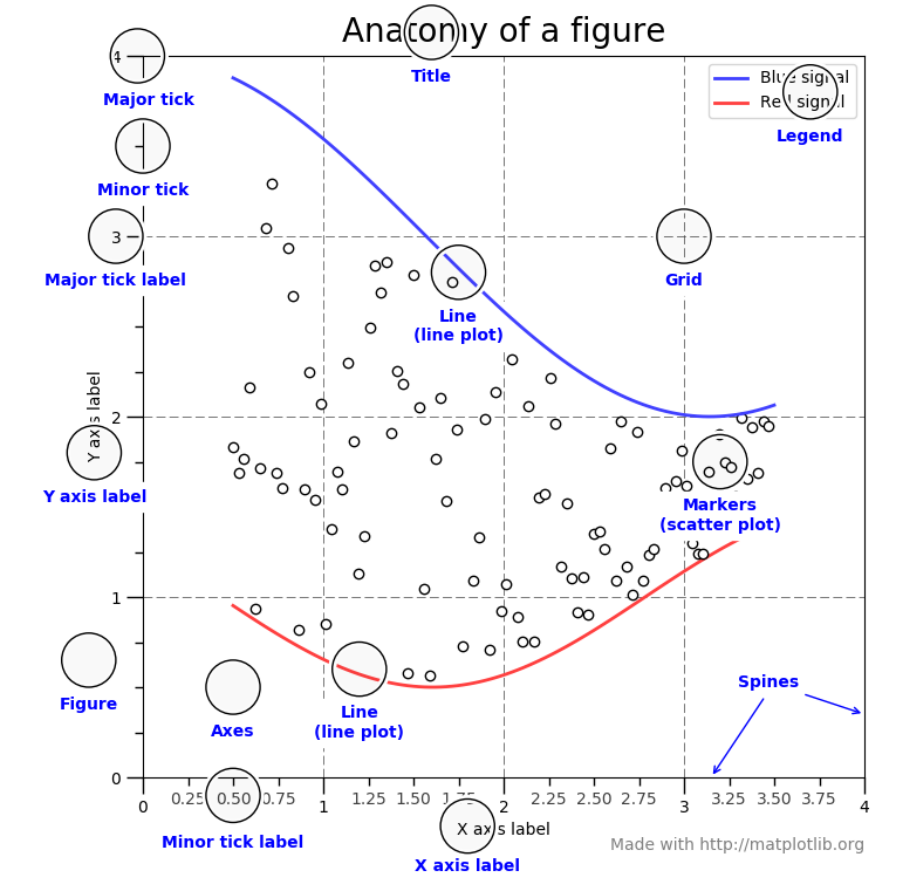
\includegraphics{images/1580807106.png}

\hypertarget{types-of-inputs-to-plotting-functions}{%
\subsubsection{Types of inputs to plotting functions}\label{types-of-inputs-to-plotting-functions}}

\begin{enumerate}
\def\labelenumi{\arabic{enumi}.}
\tightlist
\item
  All of plotting functions expect np.array or np.ma.masked\textsubscript{array} as
  input.
\item
  Classes that are 'array-like' such as pandas data objects and
  np.matrix may or may not work as intended.
\item
  It is best to convert these to np.array objects prior to plotting.
\end{enumerate}

\begin{lstlisting}[language=Python]
import matplotlib.pyplot as plt
import numpy as np
import pandas as pd

a = pd.DataFrame(np.random.rand(4,5), columns = list('abcde'))
a_asarray = a.values

b = np.matrix([[1,2],[3,4]])
b_asarray = np.asarray(b)
\end{lstlisting}

\hypertarget{matplotlib-pyplot-and-pylab-how-are-they-related}{%
\subsubsection{Matplotlib, pyplot and pylab: how are they related?}\label{matplotlib-pyplot-and-pylab-how-are-they-related}}

\begin{enumerate}
\def\labelenumi{\arabic{enumi}.}
\tightlist
\item
  Matplotlib is the whole package
\item
  and matplotlib.pyplot is a module in Matplotlib.
\item
  pylab is a convenience module that bulk imports matplotlib.pyplot
  (for plotting) and numpy (for mathematics and working with arrays)
  in a single namespace. pylab is deprecated and its use is strongly
  discouraged because of namespace pollution. Use pyplot instead.
\end{enumerate}

\hypertarget{pyplot}{%
\subsubsection{pyplot}\label{pyplot}}

\begin{enumerate}
\def\labelenumi{\arabic{enumi}.}
\tightlist
\item
  For functions in the pyplot module, there is always a "current"
  figure and axes (which is created automatically on request).
\item
  For example, in the following example, the first call to plt.plot
  creates the axes,
\item
  then subsequent calls to plt.plot add additional lines on the same
  axes,
\item
  and plt.xlabel, plt.ylabel, plt.title and plt.legend set the axes
  labels and title and add a legend.
\end{enumerate}

\begin{lstlisting}[language=Python]
x = np.linspace(0, 2, 100)

plt.plot(x, x, label='linear')
plt.plot(x, x**2, label='quadratic')
plt.plot(x, x**3, label='cubic')

plt.xlabel('x label')
plt.ylabel('y label')
plt.title("Simple Plot")
plt.legend()

plt.show()
\end{lstlisting}

\begin{center}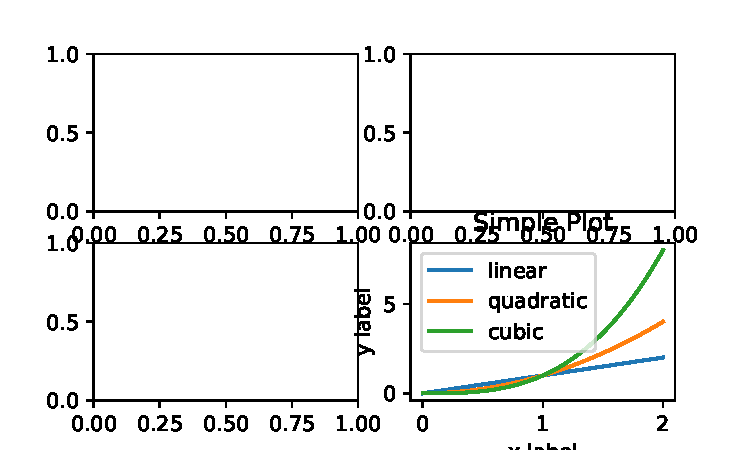
\includegraphics[width=0.9\linewidth]{python-visualization_files/figure-latex/unnamed-chunk-3-1} \end{center}

\hypertarget{ux540eux7aef}{%
\subsection{后端}\label{ux540eux7aef}}

\hypertarget{what-is-a-backend}{%
\subsubsection{What is a backend?}\label{what-is-a-backend}}

\begin{enumerate}
\def\labelenumi{\arabic{enumi}.}
\tightlist
\item
  matplotlib targets many different use cases and output formats.
\item
  To support all of these use cases, matplotlib can target different
  outputs, and each of these capabilities is called a backend;
\item
  the "frontend" is the user facing code, i.e., the plotting code,
  whereas the "backend" does all the hard work behind-the-scenes to
  make the figure.
\item
  There are two types of backends:

  \begin{enumerate}
  \def\labelenumii{\arabic{enumii}.}
  \tightlist
  \item
    user interface backends (for use in pygtk, wxpython, tkinter,
    qt4, or macosx; also referred to as "interactive backends")
  \item
    and hardcopy backends to make image files (PNG, SVG, PDF, PS;
    also referred to as "non-interactive backends").
  \end{enumerate}
\end{enumerate}

\hypertarget{configure-your-backend}{%
\subsubsection{Configure your backend}\label{configure-your-backend}}

\begin{enumerate}
\def\labelenumi{\arabic{enumi}.}
\tightlist
\item
  The backend parameter in your matplotlibrc file
\item
  If your script depends on a specific backend you can use the use()
  function.
\item
  If you use the use() function, this must be done before importing
  matplotlib.pyplot. Calling use() after pyplot has been imported will
  have no effect.
\item
  Using use() will require changes in your code if users want to use a
  different backend.
\end{enumerate}

\begin{lstlisting}[language=Python]
import matplotlib
matplotlib.use('pdf')   ### generate postscript output by default
\end{lstlisting}

\hypertarget{what-is-interactive-mode}{%
\subsubsection{What is interactive mode?}\label{what-is-interactive-mode}}

\begin{enumerate}
\def\labelenumi{\arabic{enumi}.}
\tightlist
\item
  Use of an interactive backend permits plotting to the screen.
\item
  Interactive mode may also be turned on via
  \passthrough{\lstinline!matplotlib.pyplot.ion()!},
\item
  and turned off via \passthrough{\lstinline!matplotlib.pyplot.ioff()!}.
\item
  Non-interactive example:
\end{enumerate}

\begin{lstlisting}[language=Python]
import matplotlib.pyplot as plt
plt.ioff()
plt.plot([1.6, 2.7])
\end{lstlisting}

\begin{center}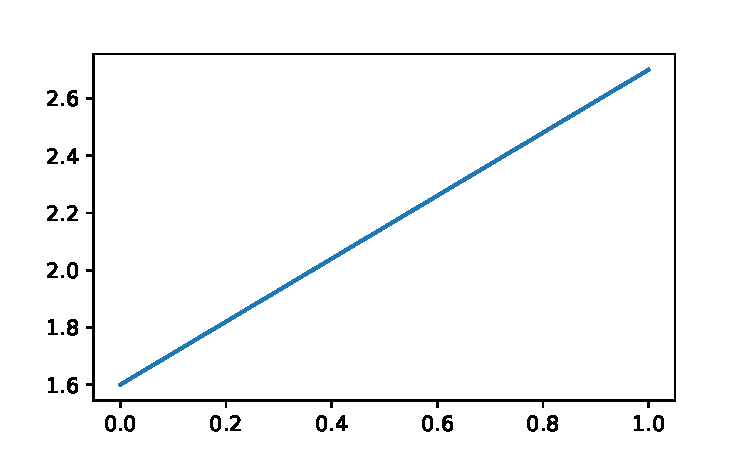
\includegraphics[width=0.9\linewidth]{python-visualization_files/figure-latex/unnamed-chunk-5-1} \end{center}

\begin{enumerate}
\def\labelenumi{\arabic{enumi}.}
\tightlist
\item
  Nothing happened--or at least nothing has shown up on the screen, To
  make the plot appear, you need to do this:
\end{enumerate}

\begin{lstlisting}[language=Python]
plt.show()
\end{lstlisting}

\begin{center}
\includegraphics[width=0.9\linewidth]{python-visualization_files/figure-latex/unnamed-chunk-6-1} \end{center}

\begin{enumerate}
\def\labelenumi{\arabic{enumi}.}
\tightlist
\item
  Now you see the plot, but your terminal command line is
  unresponsive; the \passthrough{\lstinline!show()!} command blocks the input of additional
  commands until you manually kill the plot window.
\end{enumerate}

\hypertarget{pyplot-ux7b80ux4ecb}{%
\subsection{Pyplot 简介}\label{pyplot-ux7b80ux4ecb}}

\hypertarget{intro-to-pyplot}{%
\subsubsection{Intro to pyplot}\label{intro-to-pyplot}}

\begin{enumerate}
\def\labelenumi{\arabic{enumi}.}
\tightlist
\item
  \passthrough{\lstinline!matplotlib.pyplot!} is a collection of command style functions that
  make matplotlib work like MATLAB.
\item
  Each pyplot function makes some change to a figure: e.g., creates a
  figure, creates a plotting area in a figure, plots some lines in a
  plotting area, decorates the plot with labels, etc.
\item
  In \passthrough{\lstinline!matplotlib.pyplot!} various states are preserved across function
  calls, so that it keeps track of things like the current figure and
  plotting area, and the plotting functions are directed to the
  current axes.
\item
  "axes" here and in most places in the documentation refers to the
  axes part of a figure and not the strict mathematical term for more
  than one axis.
\end{enumerate}

\hypertarget{formatting-the-style-of-your-plot}{%
\subsubsection{Formatting the style of your plot}\label{formatting-the-style-of-your-plot}}

\begin{enumerate}
\def\labelenumi{\arabic{enumi}.}
\tightlist
\item
  For every x, y pair of arguments, there is an optional third
  argument which is the format string that indicates the color and
  line type of the plot.
\item
  The letters and symbols of the format string are from MATLAB, and
  you concatenate a color string with a line style string.
\item
  The default format string is \passthrough{\lstinline!'b-'!} , which is a solid blue line.
  For example, to plot the above with red circles, use \passthrough{\lstinline!'ro'!} .
\item
  The \passthrough{\lstinline!axis()!} command in the example above takes a list of
  \passthrough{\lstinline![xmin, xmax, ymin, ymax]!} and specifies the viewport of the axes.
\end{enumerate}

\begin{lstlisting}[language=Python]
import matplotlib.pyplot as plt
plt.plot([1, 2, 3, 4], [1, 4, 9, 16], 'ro')
plt.axis([0, 6, 0, 20])
\end{lstlisting}

\begin{lstlisting}[language=Python]
plt.show()
\end{lstlisting}

\begin{center}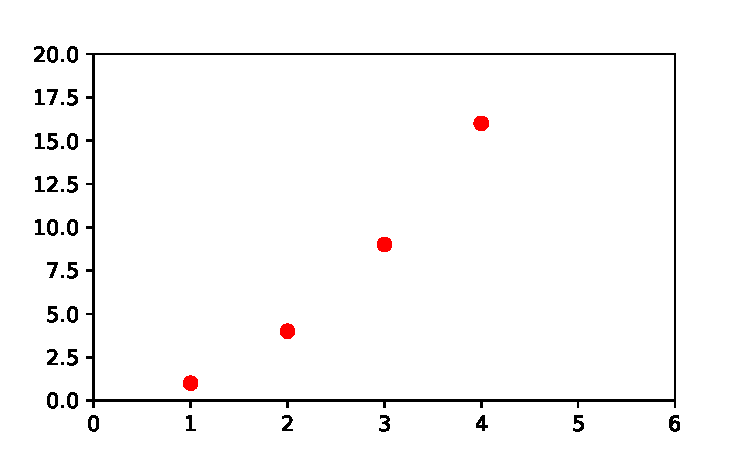
\includegraphics[width=0.9\linewidth]{python-visualization_files/figure-latex/unnamed-chunk-7-1} \end{center}

\hypertarget{use-numpy-arrays}{%
\subsubsection{use numpy arrays}\label{use-numpy-arrays}}

\begin{enumerate}
\def\labelenumi{\arabic{enumi}.}
\tightlist
\item
  matplotlib uses numpy arrays.
\item
  In fact, all sequences are converted to numpy arrays internally.
\item
  The example below illustrates a plotting several lines with
  different format styles in one command using arrays.
\end{enumerate}

\begin{lstlisting}[language=Python]
import numpy as np

# evenly sampled time at 200ms intervals
t = np.arange(0., 5., 0.2)

# red dashes, blue squares and green triangles
plt.plot(t, t, 'r--', t, t**2, 'bs', t, t**3, 'g^')
\end{lstlisting}

\begin{lstlisting}[language=Python]
plt.show()
\end{lstlisting}

\begin{center}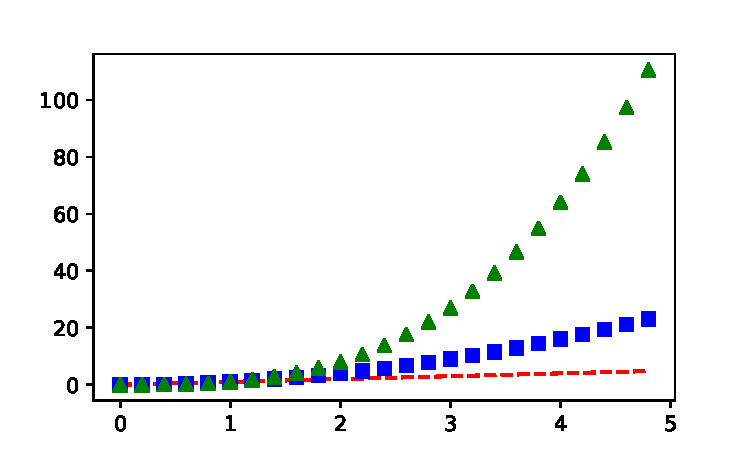
\includegraphics[width=0.9\linewidth]{python-visualization_files/figure-latex/unnamed-chunk-8-1} \end{center}

\hypertarget{plotting-with-keyword-strings}{%
\subsubsection{Plotting with keyword strings}\label{plotting-with-keyword-strings}}

\begin{enumerate}
\def\labelenumi{\arabic{enumi}.}
\tightlist
\item
  There are some instances where you have data in a format that lets
  you access particular variables with strings.
\item
  For example, \passthrough{\lstinline!pandas.DataFrame!}.
\item
  Matplotlib allows you provide such an object with the \passthrough{\lstinline!data!} keyword
  argument.
\item
  If provided, then you may generate plots with the strings
  corresponding to these variables.
\end{enumerate}

\begin{lstlisting}[language=Python]
data = {'a': np.arange(50),
        'c': np.random.randint(0, 50, 50),
        'd': np.random.randn(50)}
data['b'] = data['a'] + 10 * np.random.randn(50)
data['d'] = np.abs(data['d']) * 100

plt.scatter('a', 'b', c='c', s='d', data=data)
plt.xlabel('entry a')
plt.ylabel('entry b')
plt.show()
\end{lstlisting}

\begin{center}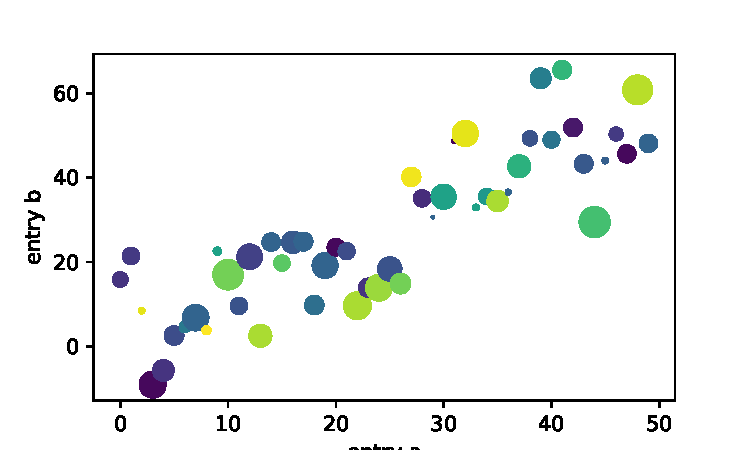
\includegraphics[width=0.9\linewidth]{python-visualization_files/figure-latex/unnamed-chunk-9-1} \end{center}

\hypertarget{plotting-with-categorical-variables}{%
\subsubsection{Plotting with categorical variables}\label{plotting-with-categorical-variables}}

\begin{enumerate}
\def\labelenumi{\arabic{enumi}.}
\tightlist
\item
  Matplotlib allows you to pass categorical variables directly to many
  plotting functions.
\end{enumerate}

\begin{lstlisting}[language=Python]
names = ['group_a', 'group_b', 'group_c']
values = [1, 10, 100]

plt.figure(figsize=(9, 3))

plt.subplot(131)
plt.bar(names, values)
\end{lstlisting}

\begin{lstlisting}[language=Python]
plt.subplot(132)
plt.scatter(names, values)
plt.subplot(133)
plt.plot(names, values)
plt.suptitle('Categorical Plotting')
plt.show()
\end{lstlisting}

\begin{center}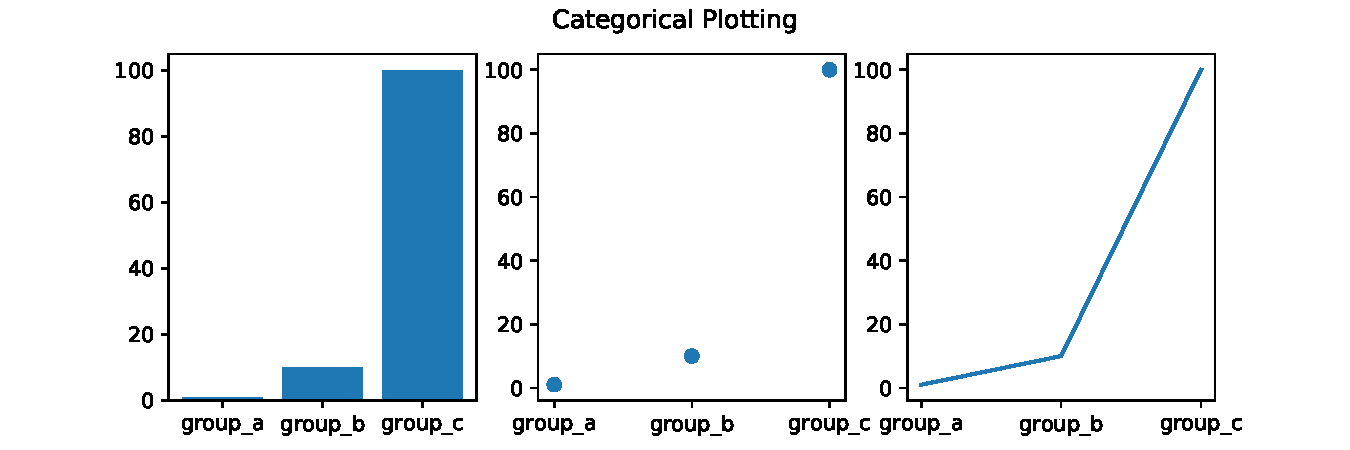
\includegraphics[width=0.9\linewidth]{python-visualization_files/figure-latex/unnamed-chunk-10-1} \end{center}

\hypertarget{ux7ebfux6761ux5c5eux6027}{%
\subsection{线条属性}\label{ux7ebfux6761ux5c5eux6027}}

\hypertarget{controlling-line-properties}{%
\subsubsection{Controlling line properties}\label{controlling-line-properties}}

\begin{enumerate}
\def\labelenumi{\arabic{enumi}.}
\tightlist
\item
  Lines have many attributes that you can set: linewidth, dash style,
  antialiased, etc; see matplotlib.lines.Line2D.
\item
  There are several ways to set line properties:

  \begin{enumerate}
  \def\labelenumii{\arabic{enumii}.}
  \tightlist
  \item
    Use keyword args: \passthrough{\lstinline!plt.plot(x, y, linewidth=2.0)!}
  \item
    Use the setter methods of a Line2D instance. plot returns a list
    of Line2D objects; e.g., line1, line2 = plot(x1, y1, x2, y2). In
    the code below we will suppose that we have only one line so
    that the list returned is of length 1. We use tuple unpacking
    with line, to get the first element of that list:
  \end{enumerate}
\end{enumerate}

\begin{lstlisting}[language=Python]
line, = plt.plot(x, y, '-')
line.set_antialiased(False) # turn off antialiasing
\end{lstlisting}

\hypertarget{controlling-line-properties-1}{%
\subsubsection{Controlling line properties}\label{controlling-line-properties-1}}

\begin{enumerate}
\def\labelenumi{\arabic{enumi}.}
\tightlist
\item
  Use the \passthrough{\lstinline!setp()!} command. The example below uses a MATLAB-style
  command to set multiple properties on a list of lines. setp works
  transparently with a list of objects or a single object. You can
  either use python keyword arguments or MATLAB-style string/value
  pairs.
\end{enumerate}

\begin{lstlisting}[language=Python]
lines = plt.plot(x1, y1, x2, y2)
# use keyword args
plt.setp(lines, color='r', linewidth=2.0)
# or MATLAB style string value pairs
plt.setp(lines, 'color', 'r', 'linewidth', 2.0)
\end{lstlisting}

\begin{enumerate}
\def\labelenumi{\arabic{enumi}.}
\tightlist
\item
  To get a list of settable line properties, call the \passthrough{\lstinline!setp()!}
  function with a line or lines as argument.
\end{enumerate}

\begin{lstlisting}[language=Python]
lines = plt.plot([1, 2, 3])
plt.setp(lines)
\end{lstlisting}

\hypertarget{ux591aux4e2aux56feux5f62ux548cux5750ux6807ux7cfb}{%
\subsection{多个图形和坐标系}\label{ux591aux4e2aux56feux5f62ux548cux5750ux6807ux7cfb}}

\hypertarget{working-with-multiple-figures-and-axes}{%
\subsubsection{Working with multiple figures and axes}\label{working-with-multiple-figures-and-axes}}

\begin{enumerate}
\def\labelenumi{\arabic{enumi}.}
\tightlist
\item
  pyplot has the concept of the current figure and the current axes.
\item
  All plotting commands apply to the current axes.
\item
  The function \passthrough{\lstinline!gca()!} returns the current axes (a
  matplotlib.axes.Axes instance),
\item
  and \passthrough{\lstinline!gcf()!} returns the current figure (matplotlib.figure.Figure
  instance).
\item
  Normally, you don't have to worry about this, because it is all
  taken care of behind the scenes.
\end{enumerate}

\begin{lstlisting}[language=Python]
def f(t):
    return np.exp(-t) * np.cos(2*np.pi*t)

t1 = np.arange(0.0, 5.0, 0.1)
t2 = np.arange(0.0, 5.0, 0.02)
plt.figure()
plt.subplot(211)
plt.plot(t1, f(t1), 'bo', t2, f(t2), 'k')
\end{lstlisting}

\begin{lstlisting}[language=Python]
plt.subplot(212)
plt.plot(t2, np.cos(2*np.pi*t2), 'r--')
plt.show()
\end{lstlisting}

\begin{center}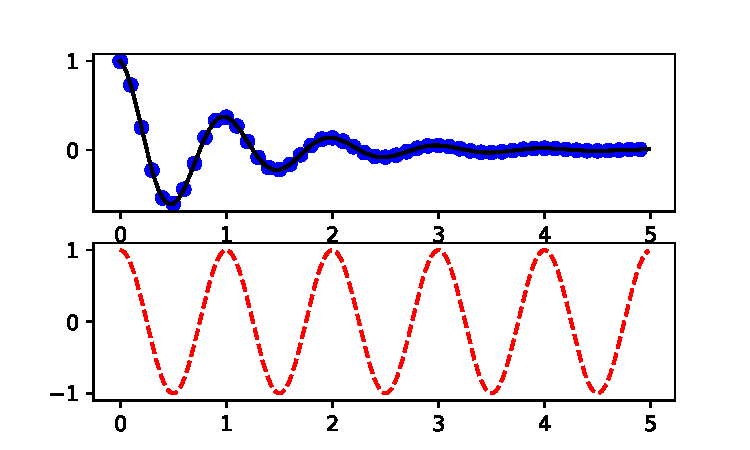
\includegraphics[width=0.9\linewidth]{python-visualization_files/figure-latex/unnamed-chunk-14-1} \end{center}

\hypertarget{working-with-multiple-figures-and-axes-1}{%
\subsubsection{Working with multiple figures and axes}\label{working-with-multiple-figures-and-axes-1}}

\begin{enumerate}
\def\labelenumi{\arabic{enumi}.}
\tightlist
\item
  The figure() command here is optional because figure(1) will be
  created by default, just as a subplot(111) will be created by
  default if you don't manually specify any axes.
\item
  The subplot() command specifies numrows, numcols, plot\textsubscript{number} where
  plot\textsubscript{number} ranges from 1 to numrows*numcols.
\item
  The commas in the subplot command are optional if
  numrows*numcols\textless{}10. So subplot(211) is identical to subplot(2, 1,
  1).
\item
  create multiple figures by using multiple figure() calls with an
  increasing figure number.
\item
  clear the current figure with clf() and the current axes with cla().
\item
  the memory required for a figure is not completely released until
  the figure is explicitly closed with close().
\end{enumerate}

\hypertarget{ux4f8bux5b50}{%
\subsubsection{例子}\label{ux4f8bux5b50}}

\begin{lstlisting}[language=Python]
import matplotlib.pyplot as plt
plt.figure(1)                # the first figure
plt.subplot(211)             # the first subplot in the first figure
plt.plot([1, 2, 3])
plt.subplot(212)             # the second subplot in the first figure
plt.plot([4, 5, 6])


plt.figure(2)                # a second figure
plt.plot([4, 5, 6])          # creates a subplot(111) by default

plt.figure(1)                # figure 1 current; subplot(212) still current
plt.subplot(211)             # make subplot(211) in figure1 current
plt.title('Easy as 1, 2, 3') # subplot 211 title
\end{lstlisting}

\begin{center}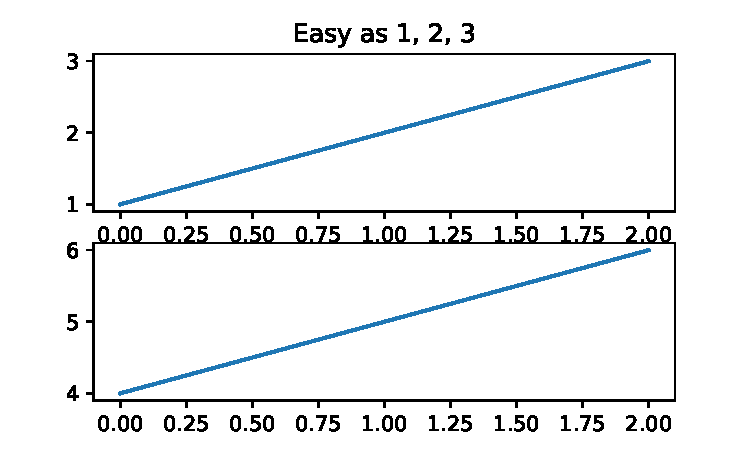
\includegraphics[width=0.9\linewidth]{python-visualization_files/figure-latex/unnamed-chunk-15-1} \end{center}

\hypertarget{working-with-text}{%
\subsection{Working with text}\label{working-with-text}}

\hypertarget{working-with-text-1}{%
\subsubsection{Working with text}\label{working-with-text-1}}

\begin{enumerate}
\def\labelenumi{\arabic{enumi}.}
\tightlist
\item
  The text() command can be used to add text in an arbitrary location,
\item
  and the xlabel(), ylabel() and title() are used to add text in the
  indicated locations.
\item
  All of the text() commands return an matplotlib.text.Text instance.
\item
  Just as with with lines above, you can customize the properties by
  passing keyword arguments into the text functions or using setp():
\end{enumerate}

\begin{lstlisting}[language=Python]
t = plt.xlabel('my data', fontsize=14, color='red')
\end{lstlisting}

\hypertarget{ux4f8bux5b50-1}{%
\subsubsection{例子}\label{ux4f8bux5b50-1}}

\begin{lstlisting}[language=Python]
mu, sigma = 100, 15
x = mu + sigma * np.random.randn(10000)

# the histogram of the data
n, bins, patches = plt.hist(x, 50, density=1, facecolor='g', alpha=0.75)


plt.xlabel('Smarts')
plt.ylabel('Probability')
plt.title('Histogram of IQ')
plt.text(60, .025, r'$\mu=100,\ \sigma=15$')
plt.axis([40, 160, 0, 0.03])
\end{lstlisting}

\begin{lstlisting}[language=Python]
plt.grid(True)
plt.show()
\end{lstlisting}

\begin{center}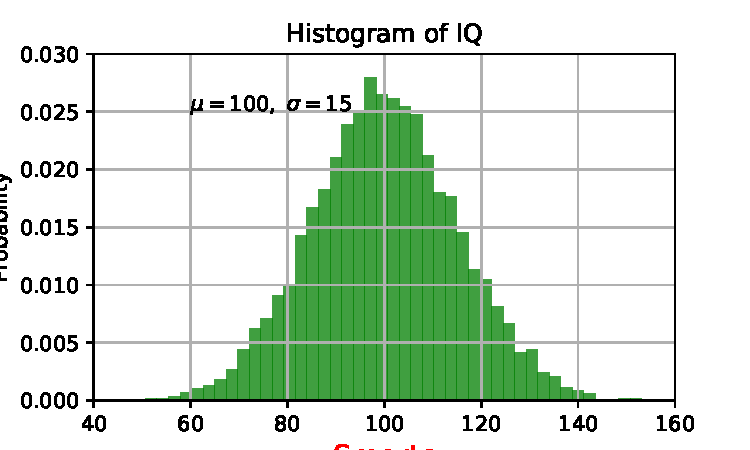
\includegraphics[width=0.9\linewidth]{python-visualization_files/figure-latex/unnamed-chunk-17-1} \end{center}

\hypertarget{using-mathematical-expressions-in-text}{%
\subsubsection{Using mathematical expressions in text}\label{using-mathematical-expressions-in-text}}

\begin{enumerate}
\def\labelenumi{\arabic{enumi}.}
\tightlist
\item
  matplotlib accepts TeX equation expressions in any text expression.
\end{enumerate}

\begin{lstlisting}[language=Python]
plt.title(r'$\sigma_i=15$')
\end{lstlisting}

\begin{center}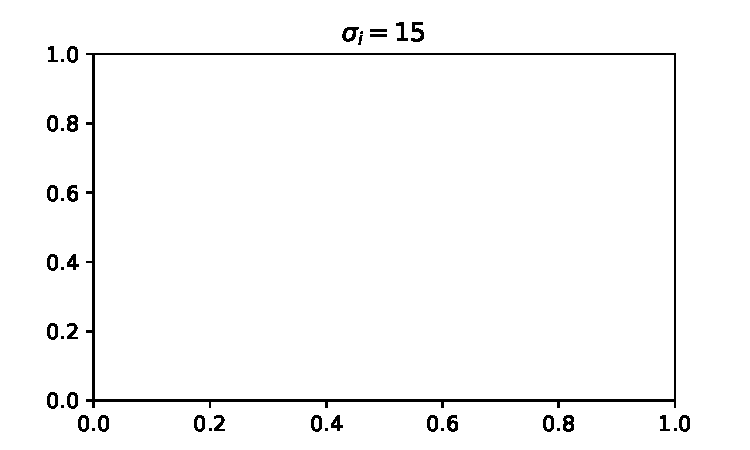
\includegraphics[width=0.9\linewidth]{python-visualization_files/figure-latex/unnamed-chunk-18-1} \end{center}

\begin{enumerate}
\def\labelenumi{\arabic{enumi}.}
\tightlist
\item
  The r preceding the title string is important -- it signifies
  that the string is a raw string and not to treat backslashes as
  python escapes.
\item
  matplotlib has a built-in TeX expression parser and layout engine,
  and ships its own math fonts. Thus you can use mathematical text
  across platforms without requiring a TeX installation.
\item
  For those who have LaTeX and dvipng installed, you can also use
  LaTeX to format your text and incorporate the output directly into
  your display figures or saved postscript
\end{enumerate}

\hypertarget{annotating-text}{%
\subsubsection{Annotating text}\label{annotating-text}}

\begin{enumerate}
\def\labelenumi{\arabic{enumi}.}
\tightlist
\item
  A common use for text is to annotate some feature of the plot, and
  the annotate() method provides helper functionality to make
  annotations easy.
\item
  In an annotation, there are two points to consider:

  \begin{enumerate}
  \def\labelenumii{\arabic{enumii}.}
  \tightlist
  \item
    the location being annotated represented by the argument xy
  \item
    and the location of the text xytext.
  \item
    Both of these arguments are (x,y) tuples.
  \end{enumerate}
\end{enumerate}

\hypertarget{ux4f8bux5b50-2}{%
\subsubsection{例子}\label{ux4f8bux5b50-2}}

\begin{lstlisting}[language=Python]
ax = plt.subplot(111)

t = np.arange(0.0, 5.0, 0.01)
s = np.cos(2*np.pi*t)
line, = plt.plot(t, s, lw=2)

plt.annotate('local max', xy=(2, 1), xytext=(3, 1.5),
             arrowprops=dict(facecolor='black', shrink=0.05),
             )

plt.ylim(-2, 2)
\end{lstlisting}

\begin{lstlisting}[language=Python]
plt.show()
\end{lstlisting}

\begin{center}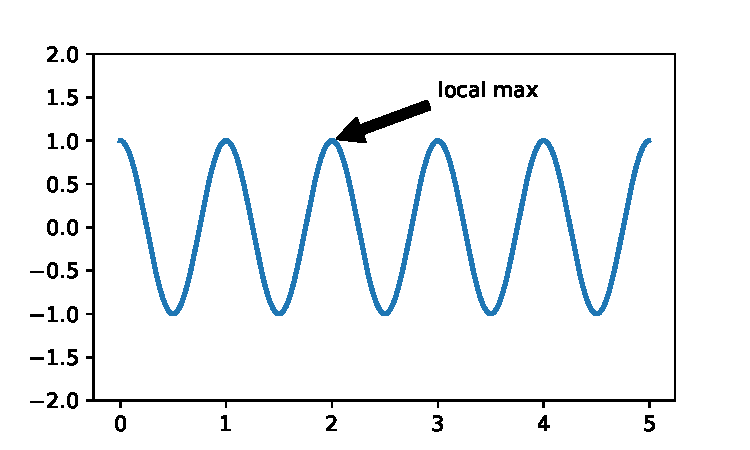
\includegraphics[width=0.9\linewidth]{python-visualization_files/figure-latex/unnamed-chunk-19-1} \end{center}

\hypertarget{ux9762ux5411ux5bf9ux8c61api}{%
\section{面向对象API}\label{ux9762ux5411ux5bf9ux8c61api}}

\hypertarget{the-object-oriented-api-vs-pyplot}{%
\subsubsection{the Object-Oriented API vs Pyplot}\label{the-object-oriented-api-vs-pyplot}}

\begin{enumerate}
\def\labelenumi{\arabic{enumi}.}
\tightlist
\item
  Matplotlib has two interfaces. The first is an object-oriented (OO)
  interface. In this case, we utilize an instance of axes.Axes in
  order to render visualizations on an instance of figure.Figure.
\item
  The second is based on MATLAB and uses a state-based interface. This
  is encapsulated in the pyplot module.
\item
  Most of the terms are straightforward but the main thing to remember
  is that:

  \begin{enumerate}
  \def\labelenumii{\arabic{enumii}.}
  \tightlist
  \item
    The Figure is the final image that may contain 1 or more Axes.
  \item
    The Axes represent an individual plot (don't confuse this with
    the word "axis", which refers to the x/y axis of a plot).
  \item
    We call methods that do the plotting directly from the Axes,
    which gives us much more flexibility and power in customizing
    our plot.
  \end{enumerate}
\item
  In general, try to use the object-oriented interface over the pyplot
  interface.
\end{enumerate}

\hypertarget{data}{%
\subsubsection{data}\label{data}}

\begin{lstlisting}[language=Python]
import numpy as np
import matplotlib.pyplot as plt
from matplotlib.ticker import FuncFormatter

data = {'Barton LLC': 109438.50,
        'Frami, Hills and Schmidt': 103569.59,
        'Fritsch, Russel and Anderson': 112214.71,
        'Jerde-Hilpert': 112591.43,
        'Keeling LLC': 100934.30,
        'Koepp Ltd': 103660.54,
        'Kulas Inc': 137351.96,
        'Trantow-Barrows': 123381.38,
        'White-Trantow': 135841.99,
        'Will LLC': 104437.60}

group_data = list(data.values())
group_names = list(data.keys())
group_mean = np.mean(group_data)
\end{lstlisting}

\hypertarget{figure-and-axes}{%
\subsubsection{Figure and axes}\label{figure-and-axes}}

\begin{enumerate}
\def\labelenumi{\arabic{enumi}.}
\tightlist
\item
  To do this with the object-oriented approach, we'll first generate
  an instance of figure.Figure and axes.Axes.
\item
  The Figure is like a canvas, and the Axes is a part of that canvas
  on which we will make a particular visualization.
\item
  Figures can have multiple axes on them.
\end{enumerate}

\begin{lstlisting}[language=Python]
fig, ax = plt.subplots()
\end{lstlisting}

\begin{enumerate}
\def\labelenumi{\arabic{enumi}.}
\tightlist
\item
  Now that we have an Axes instance, we can plot on top of it.
\end{enumerate}

\begin{lstlisting}[language=Python]
ax.barh(group_names, group_data)
\end{lstlisting}

\hypertarget{controlling-the-style}{%
\subsubsection{Controlling the style}\label{controlling-the-style}}

\begin{enumerate}
\def\labelenumi{\arabic{enumi}.}
\tightlist
\item
  There are many styles available in Matplotlib in order to let you
  tailor your visualization to your needs. To see a list of styles, we
  can use:
\end{enumerate}

\begin{lstlisting}[language=Python]
print(plt.style.available)
\end{lstlisting}

\begin{enumerate}
\def\labelenumi{\arabic{enumi}.}
\tightlist
\item
  You can activate a style with the following:
\end{enumerate}

\begin{lstlisting}[language=Python]
plt.style.use('ggplot')
\end{lstlisting}

\hypertarget{customizing-the-plot}{%
\subsubsection{Customizing the plot}\label{customizing-the-plot}}

\begin{enumerate}
\def\labelenumi{\arabic{enumi}.}
\tightlist
\item
  rotate the labels on the x-axis so that they show up more clearly.
\item
  We can gain access to these labels with the
  axes.Axes.get\textsubscript{xticklabels}() method:
\end{enumerate}

\begin{lstlisting}[language=Python]
fig, ax = plt.subplots()
ax.barh(group_names, group_data)
\end{lstlisting}

\begin{lstlisting}[language=Python]
labels = ax.get_xticklabels()
\end{lstlisting}

\begin{enumerate}
\def\labelenumi{\arabic{enumi}.}
\tightlist
\item
  If we'd like to set the property of many items at once, it's
  useful to use the pyplot.setp() function.
\item
  This will take a list (or many lists) of Matplotlib objects, and
  attempt to set some style element of each one.
\end{enumerate}

\begin{lstlisting}[language=Python]
fig, ax = plt.subplots()
ax.barh(group_names, group_data)
\end{lstlisting}

\begin{lstlisting}[language=Python]
labels = ax.get_xticklabels()
plt.setp(labels, rotation=45, horizontalalignment='right')
\end{lstlisting}

\hypertarget{customizing-the-plot-1}{%
\subsubsection{Customizing the plot}\label{customizing-the-plot-1}}

\begin{enumerate}
\def\labelenumi{\arabic{enumi}.}
\tightlist
\item
  tell Matplotlib to automatically make room for elements in the
  figures that we create.
\item
  To do this we'll set the autolayout value of our rcParams.
\end{enumerate}

\begin{lstlisting}[language=Python]
plt.rcParams.update({'figure.autolayout': True})

fig, ax = plt.subplots()
ax.barh(group_names, group_data)
\end{lstlisting}

\begin{lstlisting}[language=Python]
labels = ax.get_xticklabels()
plt.setp(labels, rotation=45, horizontalalignment='right')
\end{lstlisting}

\begin{enumerate}
\def\labelenumi{\arabic{enumi}.}
\tightlist
\item
  add labels to the plot. To do this with the OO interface, we can use
  the axes.Axes.set() method to set properties of this Axes object.
\item
  adjust the size of this plot using the pyplot.subplots() function.
  We can do this with the figsize kwarg.
\item
  For labels, we can specify custom formatting guidelines in the form
  of functions by using the ticker.FuncFormatter class.
\end{enumerate}

\hypertarget{customizing-the-plot-2}{%
\subsubsection{Customizing the plot}\label{customizing-the-plot-2}}

\begin{lstlisting}[language=Python]
def currency(x, pos):
    """The two args are the value and tick position"""
    if x >= 1e6:
        s = '${:1.1f}M'.format(x*1e-6)
    else:
        s = '${:1.0f}K'.format(x*1e-3)
    return s

formatter = FuncFormatter(currency)

fig, ax = plt.subplots(figsize=(6, 8))
ax.barh(group_names, group_data)
\end{lstlisting}

\begin{lstlisting}[language=Python]
labels = ax.get_xticklabels()
plt.setp(labels, rotation=45, horizontalalignment='right')
\end{lstlisting}

\begin{lstlisting}[language=Python]
ax.set(xlim=[-10000, 140000], xlabel='Total Revenue', ylabel='Company',
       title='Company Revenue')
\end{lstlisting}

\begin{lstlisting}[language=Python]
ax.xaxis.set_major_formatter(formatter)
\end{lstlisting}

\hypertarget{combining-multiple-visualizations}{%
\subsubsection{Combining multiple visualizations}\label{combining-multiple-visualizations}}

\begin{enumerate}
\def\labelenumi{\arabic{enumi}.}
\tightlist
\item
  It is possible to draw multiple plot elements on the same instance
  of axes.Axes.
\item
  To do this we simply need to call another one of the plot methods on
  that axes object.
\end{enumerate}

\hypertarget{combining-multiple-visualizations-1}{%
\subsubsection{Combining multiple visualizations}\label{combining-multiple-visualizations-1}}

\begin{lstlisting}[language=Python]
fig, ax = plt.subplots(figsize=(8, 8))
ax.barh(group_names, group_data)
labels = ax.get_xticklabels()
plt.setp(labels, rotation=45, horizontalalignment='right')
# Add a vertical line, here we set the style in the function call
ax.axvline(group_mean, ls='--', color='r')
# Annotate new companies
for group in [3, 5, 8]:
    ax.text(145000, group, "New Company", fontsize=10,
            verticalalignment="center")
# Now we'll move our title up since it's getting a little cramped
ax.title.set(y=1.05)
ax.set(xlim=[-10000, 140000], xlabel='Total Revenue', ylabel='Company',
       title='Company Revenue')
ax.xaxis.set_major_formatter(formatter)
ax.set_xticks([0, 25e3, 50e3, 75e3, 100e3, 125e3])
fig.subplots_adjust(right=.1)
plt.show()
\end{lstlisting}

\hypertarget{saving-plots}{%
\subsubsection{Saving plots}\label{saving-plots}}

\begin{enumerate}
\def\labelenumi{\arabic{enumi}.}
\tightlist
\item
  There are many file formats we can save to in Matplotlib. To see a
  list of available options, use:
\end{enumerate}

\begin{lstlisting}[language=Python]
print(fig.canvas.get_supported_filetypes())
\end{lstlisting}

\begin{enumerate}
\def\labelenumi{\arabic{enumi}.}
\tightlist
\item
  We can then use the figure.Figure.savefig() in order to save the
  figure to disk.
\item
  Note that there are several useful flags:

  \begin{enumerate}
  \def\labelenumii{\arabic{enumii}.}
  \tightlist
  \item
    transparent=True makes the background of the saved figure
    transparent if the format supports it.
  \item
    dpi=80 controls the resolution (dots per square inch) of the
    output.
  \item
    bbox\textsubscript{inches}="tight" fits the bounds of the figure to our
    plot.
  \end{enumerate}
\end{enumerate}

\begin{lstlisting}[language=Python]
fig.savefig('sales.png', transparent=False, dpi=80, bbox_inches="tight")
\end{lstlisting}

\hypertarget{ux901aux8fc7ux6837ux5f0fux8868ux5355ux548c-rcparams-ux53c2ux6570ux63a7ux5236ux56feux5f62}{%
\section{通过样式表单和 rcParams 参数控制图形}\label{ux901aux8fc7ux6837ux5f0fux8868ux5355ux548c-rcparams-ux53c2ux6570ux63a7ux5236ux56feux5f62}}

\hypertarget{ux6837ux5f0fux8868ux5355}{%
\subsection{样式表单}\label{ux6837ux5f0fux8868ux5355}}

\hypertarget{using-style-sheets}{%
\subsubsection{Using style sheets}\label{using-style-sheets}}

\begin{enumerate}
\def\labelenumi{\arabic{enumi}.}
\tightlist
\item
  The style package adds support for easy-to-switch plotting
  "styles" with the same parameters as a \passthrough{\lstinline!matplotlib rc!} file (which
  is read at startup to configure matplotlib).
\item
  There are a number of pre-defined styles provided by Matplotlib. For
  example, there's a pre-defined style called "ggplot", which
  emulates the aesthetics of ggplot (a popular plotting package for
  R).
\end{enumerate}

\begin{lstlisting}[language=Python]
import numpy as np
import matplotlib.pyplot as plt
import matplotlib as mpl
plt.style.use('ggplot')
data = np.random.randn(50)
\end{lstlisting}

\begin{enumerate}
\def\labelenumi{\arabic{enumi}.}
\tightlist
\item
  To list all available styles, use: \passthrough{\lstinline!print(plt.style.available)!}
\end{enumerate}

\hypertarget{defining-your-own-style}{%
\subsubsection{Defining your own style}\label{defining-your-own-style}}

\begin{enumerate}
\def\labelenumi{\arabic{enumi}.}
\tightlist
\item
  You can create custom styles and use them by calling style.use with
  the path or URL to the style sheet.
\item
  Additionally, if you add your \textless{}style-name\textgreater{}.mplstyle file to
  mpl\textsubscript{configdir}/stylelib, you can reuse your custom style sheet with
  a call to style.use(\textless{}style-name\textgreater{}).
\end{enumerate}

\hypertarget{composing-styles}{%
\subsubsection{Composing styles}\label{composing-styles}}

\begin{enumerate}
\def\labelenumi{\arabic{enumi}.}
\tightlist
\item
  Style sheets are designed to be composed together.
\item
  So you can have a style sheet that customizes colors and a separate
  style sheet that alters element sizes for presentations.
\item
  These styles can easily be combined by passing a list of styles:
\item
  Note that styles further to the right will overwrite values that are
  already defined by styles on the left.
\end{enumerate}

\begin{lstlisting}[language=Python]
# plt.style.use(['dark_background', 'presentation'])
\end{lstlisting}

\hypertarget{temporary-styling}{%
\subsubsection{Temporary styling}\label{temporary-styling}}

\begin{enumerate}
\def\labelenumi{\arabic{enumi}.}
\tightlist
\item
  use a style for a specific block of code but don't want to change
  the global styling, the style package provides a context manager for
  limiting your changes to a specific scope. To isolate your styling
  changes, you can write something like the following:
\end{enumerate}

\begin{lstlisting}[language=Python]
with plt.style.context('dark_background'):
    plt.plot(np.sin(np.linspace(0, 2 * np.pi)), 'r-o')

plt.show()
\end{lstlisting}

\begin{center}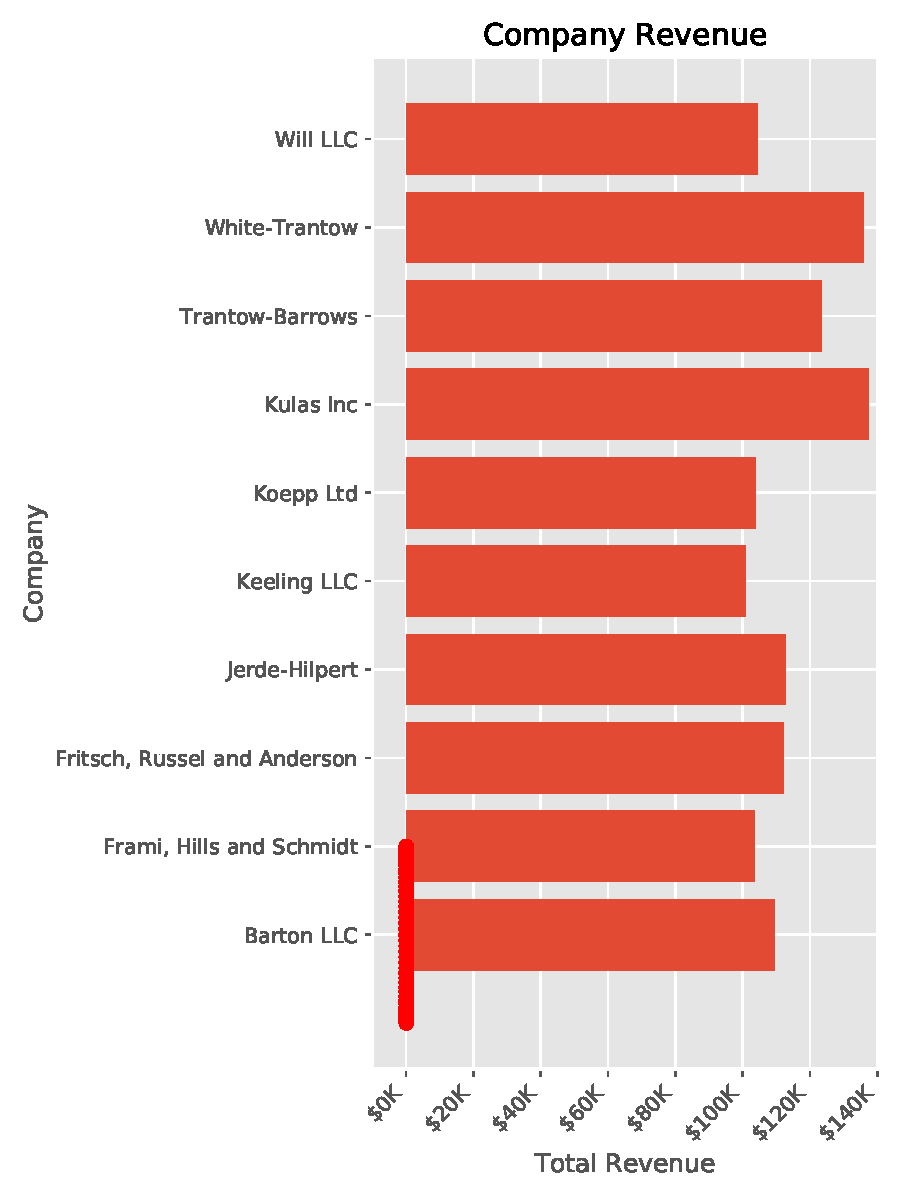
\includegraphics[width=0.9\linewidth]{python-visualization_files/figure-latex/unnamed-chunk-34-1} \end{center}

\hypertarget{rcparams-ux53c2ux6570}{%
\subsection{rcParams 参数}\label{rcparams-ux53c2ux6570}}

\hypertarget{dynamic-rc-settings}{%
\subsubsection{Dynamic rc settings}\label{dynamic-rc-settings}}

\begin{enumerate}
\def\labelenumi{\arabic{enumi}.}
\tightlist
\item
  You can also dynamically change the default rc settings in a python
  script or interactively from the python shell.
\item
  All of the rc settings are stored in a dictionary-like variable
  called matplotlib.rcParams, which is global to the matplotlib
  package.
\item
  rcParams can be modified directly, for example:
\end{enumerate}

\begin{lstlisting}[language=Python]
mpl.rcParams['lines.linewidth'] = 2
mpl.rcParams['lines.color'] = 'r'
plt.plot(data)
\end{lstlisting}

\begin{center}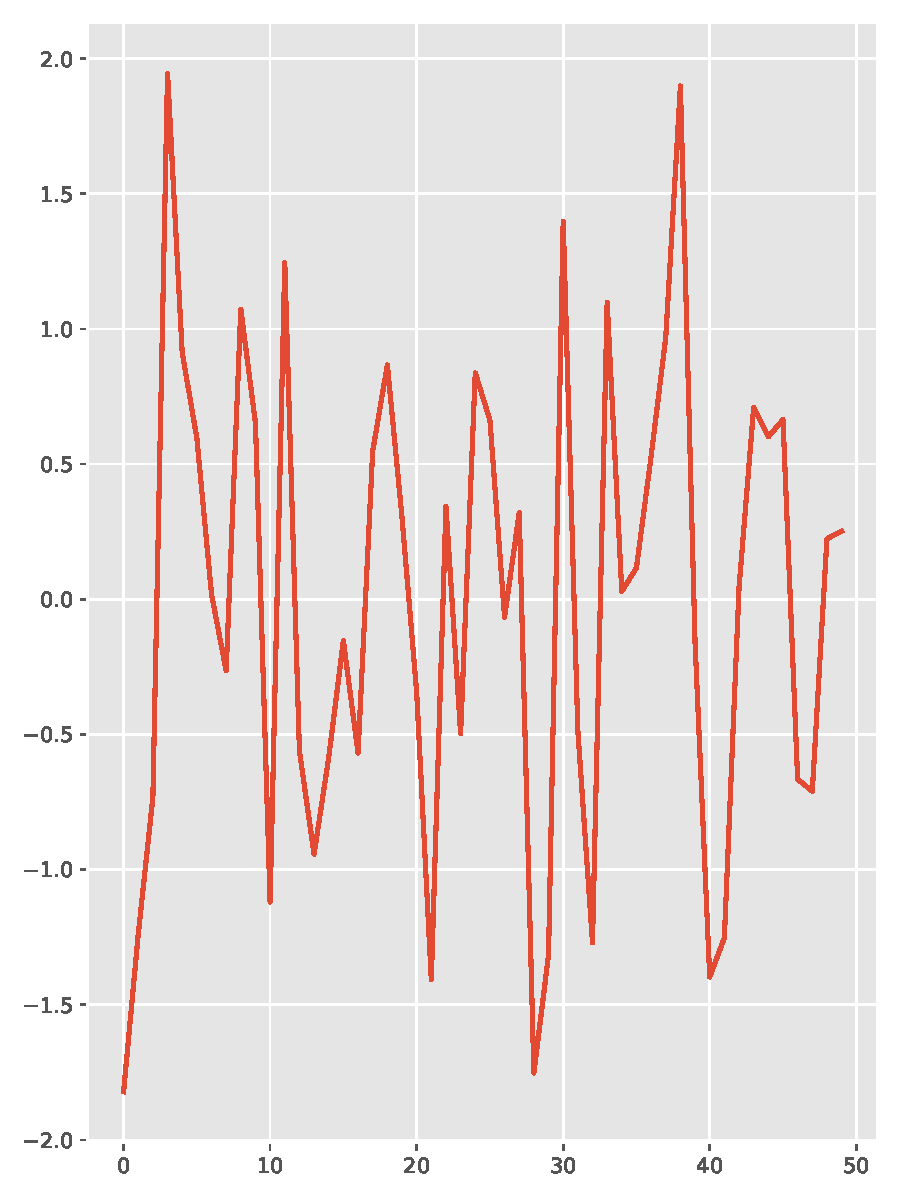
\includegraphics[width=0.9\linewidth]{python-visualization_files/figure-latex/unnamed-chunk-35-1} \end{center}

\hypertarget{dynamic-rc-settings-1}{%
\subsubsection{Dynamic rc settings}\label{dynamic-rc-settings-1}}

\begin{enumerate}
\def\labelenumi{\arabic{enumi}.}
\tightlist
\item
  Matplotlib also provides a couple of convenience functions for
  modifying rc settings. The matplotlib.rc() command can be used to
  modify multiple settings in a single group at once, using keyword
  arguments.
\item
  The matplotlib.rcdefaults() command will restore the standard
  matplotlib default settings.
\item
  There is some degree of validation when setting the values of
  rcParams, see matplotlib.rcsetup for details.
\end{enumerate}

\begin{lstlisting}[language=Python]
mpl.rc('lines', linewidth=4, color='g')
plt.plot(data)
\end{lstlisting}

\begin{center}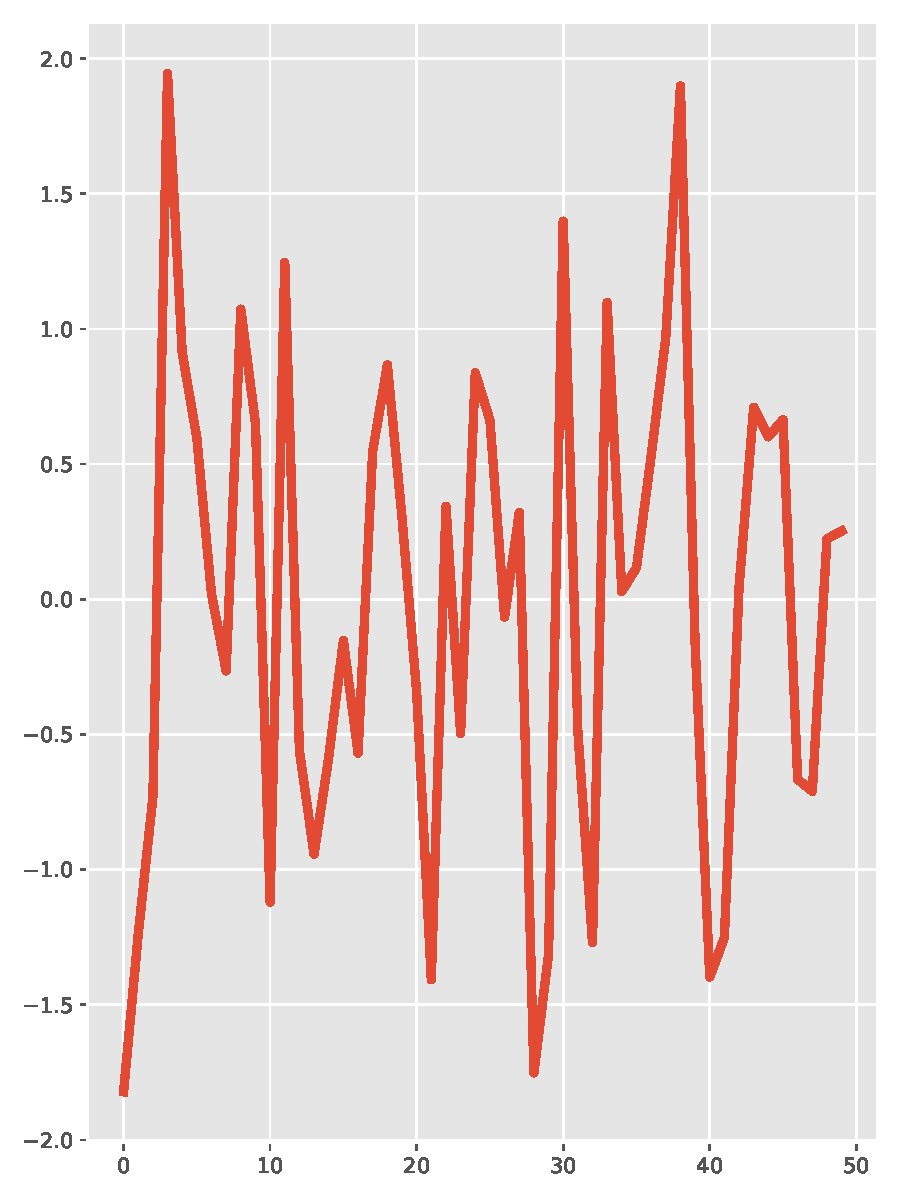
\includegraphics[width=0.9\linewidth]{python-visualization_files/figure-latex/unnamed-chunk-36-1} \end{center}

\hypertarget{the-matplotlibrc-file}{%
\subsubsection{The matplotlibrc file}\label{the-matplotlibrc-file}}

\begin{enumerate}
\def\labelenumi{\arabic{enumi}.}
\tightlist
\item
  matplotlib uses matplotlibrc configuration files to customize all
  kinds of properties, which we call rc settings or rc parameters.
\item
  You can control the defaults of almost every property in matplotlib:
  figure size and dpi, line width, color and style, axes, axis and
  grid properties, text and font properties and so on.
\item
  Once a matplotlibrc file has been found, it will not search any of
  the other paths.
\item
  To display where the currently active matplotlibrc file was loaded
  from, one can do the following:
\end{enumerate}

\begin{lstlisting}[language=Python]
import matplotlib
matplotlib.matplotlib_fname()
\end{lstlisting}

\hypertarget{artist-ux7b80ux4ecb}{%
\section{Artist 简介}\label{artist-ux7b80ux4ecb}}

\hypertarget{ux57faux672cux6982ux5ff5-1}{%
\subsection{基本概念}\label{ux57faux672cux6982ux5ff5-1}}

\hypertarget{three-layers-to-the-matplotlib-api}{%
\subsubsection{three layers to the matplotlib API}\label{three-layers-to-the-matplotlib-api}}

\begin{enumerate}
\def\labelenumi{\arabic{enumi}.}
\tightlist
\item
  the matplotlib.backend\textsubscript{bases}.FigureCanvas is the area onto which
  the figure is drawn
\item
  the matplotlib.backend\textsubscript{bases}.Renderer is the object which knows how
  to draw on the FigureCanvas
\item
  and the matplotlib.artist.Artist is the object that knows how to use
  a renderer to paint onto the canvas.
\item
  Typically, all visible elements in a figure are subclasses of
  Artist.
\end{enumerate}

\hypertarget{three-layers-to-the-matplotlib-api-1}{%
\subsubsection{three layers to the matplotlib API}\label{three-layers-to-the-matplotlib-api-1}}

\begin{enumerate}
\def\labelenumi{\arabic{enumi}.}
\tightlist
\item
  The FigureCanvas and Renderer handle all the details of talking to
  user interface toolkits like wxPython or drawing languages like
  PostScript®,
\item
  and the Artist handles all the high level constructs like
  representing and laying out the figure, text, and lines.
\item
  The typical user will spend 95\% of their time working with the
  Artists.
\end{enumerate}

\hypertarget{two-types-of-artists-primitives-and-containers}{%
\subsubsection{two types of Artists: primitives and containers}\label{two-types-of-artists-primitives-and-containers}}

\begin{enumerate}
\def\labelenumi{\arabic{enumi}.}
\tightlist
\item
  The primitives represent the standard graphical objects we want to
  paint onto our canvas: \passthrough{\lstinline!Line2D, Rectangle, Text, AxesImage!}, etc.,
\item
  and the containers are places to put them (\passthrough{\lstinline!Axis, Axes and Figure!}).
\item
  The standard use is to create a Figure instance, use the Figure to
  create one or more Axes or Subplot instances,
\item
  and use the Axes instance helper methods to create the primitives.
\end{enumerate}

\hypertarget{how-to-create-figure-instance}{%
\subsubsection{how to create Figure instance}\label{how-to-create-figure-instance}}

\begin{enumerate}
\def\labelenumi{\arabic{enumi}.}
\tightlist
\item
  we can create a Figure instance using matplotlib.pyplot.figure(),
  which is a convenience method for instantiating Figure instances and
  connecting them with your user interface or drawing toolkit
  FigureCanvas. However, this is not necessary.
\item
  you can work directly with PostScript, PDF Gtk+, or wxPython
  FigureCanvas instances, instantiate your Figures directly and
  connect them yourselves.
\end{enumerate}

\begin{lstlisting}[language=Python]
import matplotlib.pyplot as plt
fig = plt.figure()
ax = fig.add_subplot(2, 1, 1) # two rows, one column, first plot
\end{lstlisting}

\hypertarget{axes-1}{%
\subsubsection{Axes}\label{axes-1}}

\begin{enumerate}
\def\labelenumi{\arabic{enumi}.}
\tightlist
\item
  The Axes is probably the most important class in the matplotlib API,
  and the one you will be working with most of the time.
\item
  This is because the Axes is the plotting area into which most of the
  objects go,
\item
  and the Axes has many special helper methods (plot(), text(),
  hist(), imshow()) to create the most common graphics primitives
  (Line2D, Text, Rectangle, Image, respectively).
\item
  These helper methods will take your data (e.g., numpy arrays and
  strings) and create primitive Artist instances as needed (e.g.,
  Line2D), add them to the relevant containers, and draw them when
  requested.
\item
  Most of you are probably familiar with the Subplot, which is just a
  special case of an Axes that lives on a regular rows by columns grid
  of Subplot instances.
\item
  If you want to create an Axes at an arbitrary location, simply use
  the add\textsubscript{axes}() method which takes a list of \[left, bottom, width,
  height\] values in 0-1 relative figure coordinates:
\end{enumerate}

\hypertarget{ux4f8bux5b50-3}{%
\subsubsection{例子}\label{ux4f8bux5b50-3}}

\begin{lstlisting}[language=Python]
fig2 = plt.figure()
ax2 = fig2.add_axes([0.15, 0.1, 0.7, 0.3])

import numpy as np
t = np.arange(0.0, 1.0, 0.01)
s = np.sin(2*np.pi*t)
line, = ax.plot(t, s, color='blue', lw=2)

type(ax.lines)
\end{lstlisting}

\begin{lstlisting}[language=Python]
len(ax.lines)
\end{lstlisting}

\begin{lstlisting}[language=Python]
type(line)
\end{lstlisting}

\begin{enumerate}
\def\labelenumi{\arabic{enumi}.}
\tightlist
\item
  ax is the Axes instance created by the fig.add\textsubscript{subplot} call above
  (remember Subplot is just a subclass of Axes)
\item
  and when you call ax.plot, it creates a Line2D instance and adds it
  to the Axes.lines list.
\item
  remove lines by calling the list methods
\end{enumerate}

\hypertarget{ux63a7ux5236ux5bf9ux8c61}{%
\subsection{控制对象}\label{ux63a7ux5236ux5bf9ux8c61}}

\hypertarget{ux7b80ux4ecb-1}{%
\subsubsection{简介}\label{ux7b80ux4ecb-1}}

\begin{enumerate}
\def\labelenumi{\arabic{enumi}.}
\tightlist
\item
  Every element in the figure is represented by a matplotlib Artist,
\item
  and each has an extensive list of properties to configure its
  appearance.
\item
  The figure itself contains a Rectangle exactly the size of the
  figure, which you can use to set the background color and
  transparency of the figures.
\item
  each Axes bounding box (the standard white box with black edges in
  the typical matplotlib plot, has a Rectangle instance that
  determines the color, transparency, and other properties of the
  Axes.
\item
  These instances are stored as member variables \passthrough{\lstinline!Figure.patch!} and
  \passthrough{\lstinline!Axes.patch!}.
\end{enumerate}

\hypertarget{get-properties-list}{%
\subsubsection{get Properties list}\label{get-properties-list}}

\begin{enumerate}
\def\labelenumi{\arabic{enumi}.}
\tightlist
\item
  Every matplotlib Artist has many properties.
\item
  inspect the Artist properties is to use the
  \passthrough{\lstinline!matplotlib.artist.getp()!} Function (simply \passthrough{\lstinline!getp()!} in pyplot),
  which lists the properties and their values. This works for classes
  derived from Artist as well, e.g., Figure and Rectangle.
\end{enumerate}

\begin{lstlisting}[language=Python]
plt.getp(fig)
\end{lstlisting}

\begin{lstlisting}[language=Python]
plt.getp(ax)
\end{lstlisting}

\hypertarget{get-and-set-properties}{%
\subsubsection{get and set properties}\label{get-and-set-properties}}

\begin{enumerate}
\def\labelenumi{\arabic{enumi}.}
\tightlist
\item
  Each of the properties is accessed with an old-fashioned setter or
  getter.
\item
  If you want to set a number of properties at once, you can also use
  the set method with keyword arguments.
\end{enumerate}

\begin{lstlisting}[language=Python]
a = line.get_alpha()
line.set_alpha(0.5*a)

line.set(alpha=0.5, zorder=2)
\end{lstlisting}

\hypertarget{ux5bf9ux8c61ux5bb9ux5668}{%
\subsection{对象容器}\label{ux5bf9ux8c61ux5bb9ux5668}}

\hypertarget{figure-container}{%
\subsubsection{Figure container}\label{figure-container}}

\begin{enumerate}
\def\labelenumi{\arabic{enumi}.}
\tightlist
\item
  The top level container Artist is the matplotlib.figure.Figure, and
  it contains everything in the figure.
\item
  The background of the figure is a Rectangle which is stored in
  Figure.patch.
\item
  As you add subplots (add\textsubscript{subplot}()) and axes (add\textsubscript{axes}()) to the
  figure these will be appended to the Figure.axes.
\item
  Because the figure maintains the concept of the "current axes"
  (see Figure.gca and Figure.sca) to support the pyplot state machine,
  you should not insert or remove axes directly from the axes list,
  but rather use the add\textsubscript{subplot}() and add\textsubscript{axes}() methods to insert,
  and the delaxes() method to delete.
\item
  iterate over the list of axes or index into it to get access to Axes
  instances you want to customize.
\end{enumerate}

\hypertarget{ux4f8bux5b50-4}{%
\subsubsection{例子}\label{ux4f8bux5b50-4}}

\begin{lstlisting}[language=Python]
fig = plt.figure()

ax1 = fig.add_subplot(211)
ax2 = fig.add_axes([0.1, 0.1, 0.7, 0.3])
print(fig.axes)
\end{lstlisting}

\begin{lstlisting}[language=Python]
for ax in fig.axes:
    ax.grid(True)
\end{lstlisting}

\hypertarget{axes-container}{%
\subsubsection{Axes container}\label{axes-container}}

\begin{enumerate}
\def\labelenumi{\arabic{enumi}.}
\tightlist
\item
  The matplotlib.axes.Axes is the center of the matplotlib universe.
\item
  it contains the vast majority of all the Artists used in a figure
  with many helper methods to create and add these Artists to itself,
  as well as helper methods to access and customize the Artists it
  contains.
\item
  Like the Figure, it contains a Patch patch which is a Rectangle for
  Cartesian coordinates and a Circle for polar coordinates;
\item
  this patch determines the shape, background and border of the
  plotting region.
\end{enumerate}

\hypertarget{axis-containers}{%
\subsubsection{Axis containers}\label{axis-containers}}

\begin{enumerate}
\def\labelenumi{\arabic{enumi}.}
\tightlist
\item
  The matplotlib.axis.Axis instances handle the drawing of the tick
  lines, the grid lines, the tick labels and the axis label.
\item
  You can configure the left and right ticks separately for the
  y-axis, and the upper and lower ticks separately for the x-axis.
\item
  The Axis also stores the data and view intervals used in
  auto-scaling, panning and zooming, as well as the Locator and
  Formatter instances which control where the ticks are placed and how
  they are represented as strings.
\item
  Each Axis object contains a label attribute (this is what pyplot
  modifies in calls to xlabel() and ylabel()) as well as a list of
  major and minor ticks.
\item
  The ticks are XTick and YTick instances, which contain the actual
  line and text primitives that render the ticks and ticklabels.
\item
  access the lists of major and minor ticks through their accessor
  methods get\textsubscript{majorticks}() and get\textsubscript{minorticks}().
\end{enumerate}

\hypertarget{ux4f8bux5b50-5}{%
\subsubsection{例子}\label{ux4f8bux5b50-5}}

\begin{lstlisting}[language=Python]
fig, ax = plt.subplots()
axis = ax.xaxis
axis.get_ticklocs()
\end{lstlisting}

\begin{lstlisting}[language=Python]
axis.get_ticklabels()
\end{lstlisting}

\begin{lstlisting}[language=Python]
axis.get_ticklines()
\end{lstlisting}

\begin{lstlisting}[language=Python]
axis.get_ticklines(minor=True)
\end{lstlisting}

\begin{enumerate}
\def\labelenumi{\arabic{enumi}.}
\tightlist
\item
  note there are twice as many ticklines as labels because by default
  there are tick lines at the top and bottom but only tick labels
  below the xaxis.
\end{enumerate}

\hypertarget{tick-containers}{%
\subsubsection{Tick containers}\label{tick-containers}}

\begin{enumerate}
\def\labelenumi{\arabic{enumi}.}
\tightlist
\item
  The matplotlib.axis.Tick is the final container object in our
  descent from the Figure to the Axes to the Axis to the Tick.
\item
  The Tick contains the tick and grid line instances, as well as the
  label instances for the upper and lower ticks.
\item
  Each of these is accessible directly as an attribute of the Tick.
\end{enumerate}

\hypertarget{ux4f8bux5b50-6}{%
\subsubsection{例子}\label{ux4f8bux5b50-6}}

\begin{lstlisting}[language=Python]
np.random.seed(19680801)

fig, ax = plt.subplots()
ax.plot(100*np.random.rand(20))

formatter = ticker.FormatStrFormatter('$%1.2f')
ax.yaxis.set_major_formatter(formatter)

for tick in ax.yaxis.get_major_ticks():
    tick.label1.set_visible(False)
    tick.label2.set_visible(True)
    tick.label2.set_color('green')

plt.show()
\end{lstlisting}

\hypertarget{ux56feux4f8b}{%
\section{图例}\label{ux56feux4f8b}}

\hypertarget{ux4e09ux79cdux7528ux6cd5}{%
\subsubsection{三种用法}\label{ux4e09ux79cdux7528ux6cd5}}

\begin{enumerate}
\def\labelenumi{\arabic{enumi}.}
\tightlist
\item
  \passthrough{\lstinline!legend()!}
\item
  \passthrough{\lstinline!legend(labels)!}
\item
  \passthrough{\lstinline!legend(handles, labels)!}
\end{enumerate}

\hypertarget{automatic-detection-of-elements-to-be-shown-in-the-legend}{%
\subsubsection{Automatic detection of elements to be shown in the legend}\label{automatic-detection-of-elements-to-be-shown-in-the-legend}}

\begin{enumerate}
\def\labelenumi{\arabic{enumi}.}
\tightlist
\item
  The elements to be added to the legend are automatically determined,
  when you do not pass in any extra arguments.
\item
  In this case, the labels are taken from the artist.
\item
  You can specify them either at artist creation or by calling the
  set\textsubscript{label}() method on the artist.
\item
  Specific lines can be excluded from the automatic legend element
  selection by defining a label starting with an underscore.
\item
  This is default for all artists, so calling Axes.legend without any
  arguments and without setting the labels manually will result in no
  legend being drawn.
\end{enumerate}

\hypertarget{ux4f8bux5b50-7}{%
\subsubsection{例子}\label{ux4f8bux5b50-7}}

\begin{lstlisting}[language=Python]
line, = ax.plot([1, 2, 3], label='Inline label')
ax.legend()

line, = ax.plot([1, 2, 3])
line.set_label('Label via method')
ax.legend()
\end{lstlisting}

\begin{center}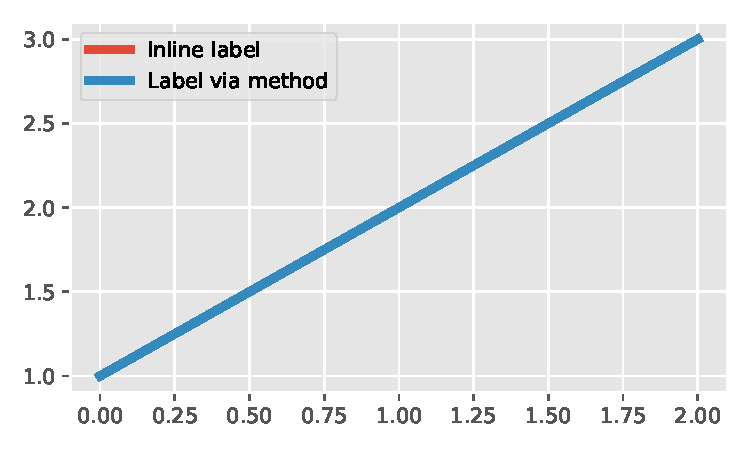
\includegraphics[width=0.9\linewidth]{python-visualization_files/figure-latex/unnamed-chunk-45-1} \end{center}

\hypertarget{labeling-existing-plot-elements}{%
\subsubsection{Labeling existing plot elements}\label{labeling-existing-plot-elements}}

\begin{enumerate}
\def\labelenumi{\arabic{enumi}.}
\tightlist
\item
  To make a legend for lines which already exist on the axes (via plot
  for instance), simply call this function with an iterable of
  strings, one for each legend item.
\item
  Note: This way of using is discouraged, because the relation between
  plot elements and labels is only implicit by their order and can
  easily be mixed up.
\end{enumerate}

\begin{lstlisting}[language=Python]
ax.plot([1, 2, 3])
ax.legend(['A simple line'])
\end{lstlisting}

\begin{center}
\includegraphics[width=0.9\linewidth]{python-visualization_files/figure-latex/unnamed-chunk-46-1} \end{center}

\hypertarget{explicitly-defining-the-elements-in-the-legend}{%
\subsubsection{Explicitly defining the elements in the legend}\label{explicitly-defining-the-elements-in-the-legend}}

\begin{enumerate}
\def\labelenumi{\arabic{enumi}.}
\tightlist
\item
  For full control of which artists have a legend entry, it is
  possible to pass an iterable of legend artists followed by an
  iterable of legend labels respectively.
\end{enumerate}

\passthrough{\lstinline!legend((line1, line2, line3), ('label1', 'label2', 'label3'))!}

\begin{enumerate}
\def\labelenumi{\arabic{enumi}.}
\tightlist
\item
  Parameters:

  \begin{enumerate}
  \def\labelenumii{\arabic{enumii}.}
  \tightlist
  \item
    loc : The location of the legend. 'best'
  \item
    bbox\textsubscript{toanchor}: Box that is used to position the legend in
    conjunction with loc.
  \item
    fontsize
  \end{enumerate}
\end{enumerate}

\hypertarget{ux4f8bux5b50-8}{%
\subsubsection{例子}\label{ux4f8bux5b50-8}}

\begin{enumerate}
\def\labelenumi{\arabic{enumi}.}
\tightlist
\item
  Examples using matplotlib.pyplot.legend,更多例子见:
  \url{https://matplotlib.org/api/_as_gen/matplotlib.pyplot.legend.html\#matplotlib.pyplot.legend}
\end{enumerate}

\begin{lstlisting}[language=Python]
import numpy as np
import matplotlib.pyplot as plt
# Make some fake data.
a = b = np.arange(0, 3, .02)
c = np.exp(a)
d = c[::-1]
# Create plots with pre-defined labels.
fig, ax = plt.subplots()
ax.plot(a, c, 'k--', label='Model length')
ax.plot(a, d, 'k:', label='Data length')
ax.plot(a, c + d, 'k', label='Total message length')
legend = ax.legend(loc='upper center', shadow=True, fontsize='x-large')
# Put a nicer background color on the legend.
legend.get_frame().set_facecolor('C0')

plt.show()
\end{lstlisting}

\begin{center}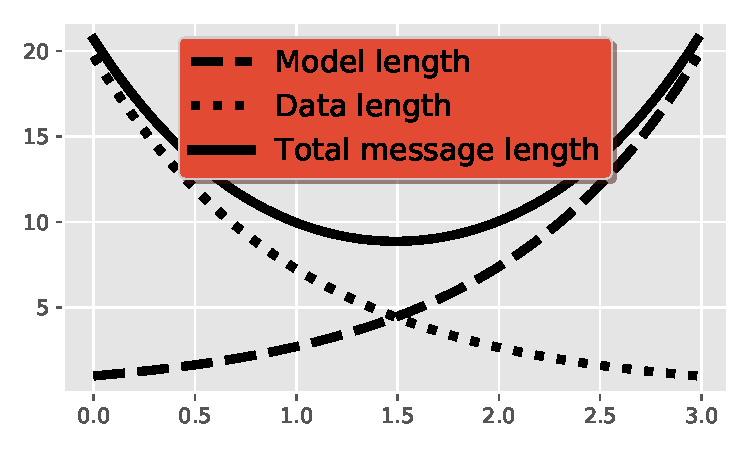
\includegraphics[width=0.9\linewidth]{python-visualization_files/figure-latex/unnamed-chunk-47-1} \end{center}

\hypertarget{ux7d27ux7f29ux8f93ux51faux548cux9650ux5b9aux8f93ux51fa}{%
\section{紧缩输出和限定输出}\label{ux7d27ux7f29ux8f93ux51faux548cux9650ux5b9aux8f93ux51fa}}

\hypertarget{tight-layout}{%
\subsubsection{Tight Layout}\label{tight-layout}}

\begin{enumerate}
\def\labelenumi{\arabic{enumi}.}
\tightlist
\item
  tight\textsubscript{layout} automatically adjusts subplot params so that the
  subplot(s) fits in to the figure area.
\item
  tight\textsubscript{layout}() only considers ticklabels, axis labels, and titles.
  Thus, other artists may be clipped and also may overlap.
\item
  An alternative to tight\textsubscript{layout} is constrained\textsubscript{layout}.
\item
  To prevent this, the location of axes needs to be adjusted. For
  subplots, this can be done by adjusting the subplot params (Move the
  edge of an axes to make room for tick labels).
\item
  \passthrough{\lstinline!tight\_layout()!} that does this automatically for you.
\item
  Note that \passthrough{\lstinline!matplotlib.pyplot.tight\_layout()!} will only adjust the
  subplot params when it is called.
\item
  In order to perform this adjustment each time the figure is redrawn,
  you can call \passthrough{\lstinline!fig.set\_tight\_layout(True)!}, or, equivalently, set the
  figure.autolayout rcParam to True.
\end{enumerate}

\hypertarget{ux4f8bux5b50-9}{%
\subsubsection{例子}\label{ux4f8bux5b50-9}}

\begin{lstlisting}[language=Python]
import matplotlib.pyplot as plt
import numpy as np
plt.rcParams['savefig.facecolor'] = "0.8"

def example_plot(ax, fontsize=12):
    ax.plot([1, 2])

    ax.locator_params(nbins=3)
    ax.set_xlabel('x-label', fontsize=fontsize)
    ax.set_ylabel('y-label', fontsize=fontsize)
    ax.set_title('Title', fontsize=fontsize)

plt.close('all')
fig, ax = plt.subplots()
example_plot(ax, fontsize=24)

fig, ax = plt.subplots()
example_plot(ax, fontsize=24)
plt.tight_layout()
\end{lstlisting}

\hypertarget{multiple-subplots}{%
\subsubsection{multiple subplots}\label{multiple-subplots}}

\begin{enumerate}
\def\labelenumi{\arabic{enumi}.}
\tightlist
\item
  When you have multiple subplots, often you see labels of different
  axes overlapping each other.
\item
  tight\textsubscript{layout}() will also adjust spacing between subplots to
  minimize the overlaps.
\item
  tight\textsubscript{layout}() will work even if the sizes of subplots are
  different as far as their grid specification is compatible.
\end{enumerate}

\hypertarget{ux4f8bux5b50-10}{%
\subsubsection{例子}\label{ux4f8bux5b50-10}}

\begin{lstlisting}[language=Python]
plt.close('all')
fig = plt.figure()

ax1 = plt.subplot(221)
ax2 = plt.subplot(223)
ax3 = plt.subplot(122)

example_plot(ax1)
example_plot(ax2)
example_plot(ax3)

plt.tight_layout()
\end{lstlisting}

\hypertarget{constrained-layout}{%
\subsubsection{Constrained Layout}\label{constrained-layout}}

\begin{enumerate}
\def\labelenumi{\arabic{enumi}.}
\tightlist
\item
  constrained\textsubscript{layout} automatically adjusts subplots and decorations
  like legends and colorbars so that they fit in the figure window
  while still preserving, as best they can, the logical layout
  requested by the user.
\item
  constrained\textsubscript{layout} is similar to tight\textsubscript{layout}, but uses a
  constraint solver to determine the size of axes that allows them to
  fit.
\item
  constrained\textsubscript{layout} needs to be activated before any axes are added
  to a figure. Two ways of doing so are

  \begin{enumerate}
  \def\labelenumii{\arabic{enumii}.}
  \tightlist
  \item
    using the respective argument to subplots() or figure(), e.g.:
    \passthrough{\lstinline!plt.subplots(constrained\_layout=True)!}
  \item
    activate it via rcParams, like:
    \passthrough{\lstinline!plt.rcParams['figure.constrained\_layout.use'] = True!}
  \end{enumerate}
\end{enumerate}

\hypertarget{ux4f8bux5b50-11}{%
\subsubsection{例子}\label{ux4f8bux5b50-11}}

\begin{lstlisting}[language=Python]
fig, ax = plt.subplots(constrained_layout=False)
example_plot(ax, fontsize=24)

fig, ax = plt.subplots(constrained_layout=True)
example_plot(ax, fontsize=24)

fig, axs = plt.subplots(2, 2, constrained_layout=False)
for ax in axs.flat:
    example_plot(ax)

fig, axs = plt.subplots(2, 2, constrained_layout=True)
for ax in axs.flat:
    example_plot(ax)
\end{lstlisting}

\hypertarget{ux56feux5f62ux4e2dux7684ux6587ux672c}{%
\section{图形中的文本}\label{ux56feux5f62ux4e2dux7684ux6587ux672c}}

\hypertarget{ux7b80ux4ecb-2}{%
\subsubsection{简介}\label{ux7b80ux4ecb-2}}

\begin{enumerate}
\def\labelenumi{\arabic{enumi}.}
\item
  Matplotlib具有广泛的文本支持,包括对数学表达式的支持、对光栅和向量输出的字体支持、带有任意旋转的换行分隔文本以及字符编码支持
\item
  Matplotlib包含自己的Matplotlib.font\_manager模块,可以实现跨平台、W3C兼容的字体查找算法。
\item
  用户对文本属性(字体大小,字体的粗细,文字的位置和颜色等)有很大的控制权,可以通过rc文件进行合理的修改。值得注意的是,对于那些对数学或科学图形感兴趣的人,Matplotlib实现了大量TeX数学符号和命令,支持图形中的任何数学表达式。
\end{enumerate}

\hypertarget{basic-text-commands}{%
\subsubsection{Basic text commands}\label{basic-text-commands}}

\begin{longtable}[]{@{}lll@{}}
\toprule
pyplot API & OO API & description\tabularnewline
\midrule
\endhead
text & text & 在轴的任意位置添加文本。\tabularnewline
annotate & annotate & 在坐标轴的任意位置添加带有可选箭头的注释。\tabularnewline
xlabel & set\textsubscript{xlabel} & 在坐标轴的x轴上添加一个标签。\tabularnewline
ylabel & set\textsubscript{ylabel} & 在坐标轴的y轴上添加一个标签。\tabularnewline
title & set\textsubscript{title} & 给这些轴添加一个标题。\tabularnewline
figtext & text & 在图形的任意位置添加文本。\tabularnewline
suptitle & suptitle & 给图添加一个标题。\tabularnewline
\bottomrule
\end{longtable}

\begin{itemize}
\tightlist
\item
  所有这些函数都创建并返回一个文本实例,该实例可以配置为各种字体和其他属性。
\end{itemize}

\hypertarget{ux4f8bux5b50-12}{%
\subsubsection{例子}\label{ux4f8bux5b50-12}}

\begin{lstlisting}[language=Python]
import matplotlib
import matplotlib.pyplot as plt

fig = plt.figure()
ax = fig.add_subplot(111)
fig.subplots_adjust(top=0.85) #(调整图形高度)
# Set titles for the figure and the subplot respectively
fig.suptitle('bold figure suptitle', fontsize=14, fontweight='bold') # 添加图标题
ax.set_title('axes title')  #添加轴标题
ax.set_xlabel('xlabel')  # 添加轴标签
ax.set_ylabel('ylabel')  # 添加轴标签
# Set both x- and y-axis limits to [0, 10] instead of default [0, 1]
ax.axis([0, 10, 0, 10]) # 修改轴坐标范围
\end{lstlisting}

\begin{lstlisting}[language=Python]
ax.text(3, 8, 'boxed italics text in data coords', style='italic',
        bbox={'facecolor': 'red', 'alpha': 0.5, 'pad': 10}) # 在指定位置添加文本,alpha对应透明度,pad对应图形宽度
ax.text(3, 2, 'unicode: Institut für Festkörperphysik')
ax.text(0.95, 0.01, 'colored text in axes coords',
        verticalalignment='bottom', horizontalalignment='right',
        transform=ax.transAxes,
        color='green', fontsize=15)

ax.plot([2], [1], 'o')
ax.annotate('annotate', xy=(2, 1), xytext=(3, 4),
            arrowprops=dict(facecolor='black', shrink=0.05)) # shrink箭头长短
plt.show()
\end{lstlisting}

\begin{center}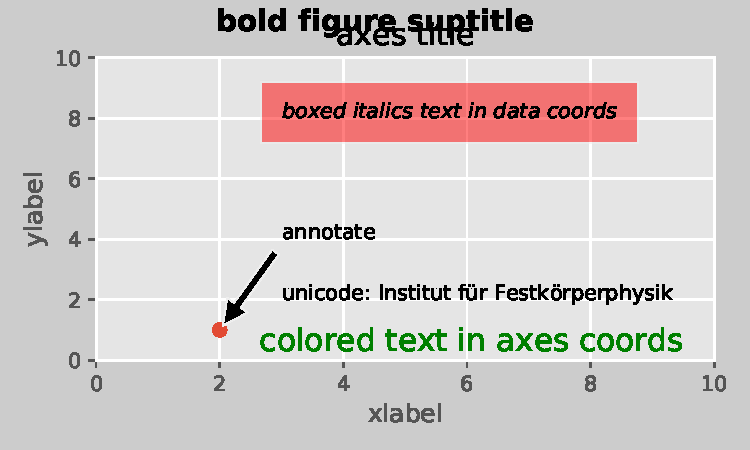
\includegraphics[width=0.9\linewidth]{python-visualization_files/figure-latex/unnamed-chunk-51-1} \end{center}

\begin{lstlisting}[language=Python]
plt.getp(ax.texts)
\end{lstlisting}

\hypertarget{text-properties-and-layout}{%
\subsubsection{Text properties and layout}\label{text-properties-and-layout}}

\begin{enumerate}
\def\labelenumi{\arabic{enumi}.}
\tightlist
\item
  matplotlib.text文本实例具有各种属性
\item
  这些属性可以通过文本命令的关键字参数(例如,title()、xlabel()和text())来配置
\item
  通过``pl .getp(ax.text)''获取属性列表
\end{enumerate}

\hypertarget{default-font}{%
\subsubsection{Default Font}\label{default-font}}

\begin{enumerate}
\def\labelenumi{\arabic{enumi}.}
\tightlist
\item
  基本默认字体由一组rcParams控制。
\end{enumerate}

\begin{longtable}[]{@{}ll@{}}
\toprule
rcParam & usage\tabularnewline
\midrule
\endhead
'font.family' & 字体名称列表,例如\{'cursive', 'fantasy', 'monospace', 'sans', 'sans serif', 'sans-serif', 'serif'\}.\tabularnewline
'font.style' & 默认样式, 例如 'normal', 'italic'.\tabularnewline
'font.variant' & 默认变体, ex 'normal', 'small-caps' (untested)\tabularnewline
'font.stretch' & 默认延伸, ex 'normal', 'condensed' (incomplete)\tabularnewline
'font.weight' & 默认空间大小。字符串或整数\tabularnewline
'font.size' & 默认字体大小(以点为单位)。相对字体大小 ('large', 'x-small') 是根据这个大小计算的。\tabularnewline
\bottomrule
\end{longtable}

\hypertarget{text-with-non-latin-glyphs}{%
\subsubsection{Text with non-latin glyphs}\label{text-with-non-latin-glyphs}}

\begin{enumerate}
\def\labelenumi{\arabic{enumi}.}
\tightlist
\item
  Matplotlib仍然没有覆盖用户可能需要的所有符号。
\item
  例如,DejaVu没有覆盖中文、韩语或日语。
\item
  将默认字体设置修改为支持所需字体,将字体名称前置到'font.family~或列表中。

  \begin{enumerate}
  \def\labelenumii{\arabic{enumii}.}
  \tightlist
  \item
    \passthrough{\lstinline!matplotlib.rcParams['font.sans-serif'] = ['SimHei', 'sans-serif']!}
  \item
    or set it in your .matplotlibrc file:
    \passthrough{\lstinline!font.sans-serif: SimHei, Arial, sans-serif!}
  \end{enumerate}
\end{enumerate}

\hypertarget{ux6807ux6ce8}{%
\section{标注}\label{ux6807ux6ce8}}

\hypertarget{ux57faux672cux6807ux6ce8}{%
\subsection{基本标注}\label{ux57faux672cux6807ux6ce8}}

\hypertarget{basic-annotation}{%
\subsubsection{Basic annotation}\label{basic-annotation}}

\begin{enumerate}
\def\labelenumi{\arabic{enumi}.}
\tightlist
\item
  用户使用text(),可以将文本放在坐标轴中的任意位置。
\item
  文本常用于注释图形的一些特性,而annotate()方法提供了辅助功能,使注释更容易
\item
  在注释中,有两点需要考虑:由参数xy表示的被注释的位置和由xytext表示的文本的位置。
\item
  这两个参数都是(x,y)元组。
\end{enumerate}

\hypertarget{basic-annotation-1}{%
\subsubsection{Basic annotation}\label{basic-annotation-1}}

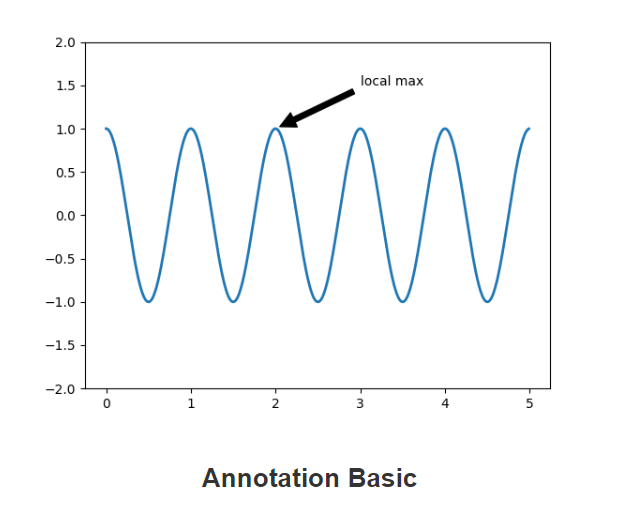
\includegraphics{images/1581585591.png}

\hypertarget{coordinate-systems}{%
\subsubsection{coordinate systems}\label{coordinate-systems}}

\begin{enumerate}
\def\labelenumi{\arabic{enumi}.}
\tightlist
\item
  有各种各样的坐标系可供选择。
\item
  可以使用以下xycoords和textcoords的字符串来指定xy和xytext的位置。
\item
  (默认是 'data')
\end{enumerate}

\begin{longtable}[]{@{}ll@{}}
\toprule
argument & coordinate system\tabularnewline
\midrule
\endhead
'figure points' & point 从图的左下角开始\tabularnewline
'figure pixels' & pixels 从图的左下角开始\tabularnewline
'figure fraction' & 0,0 是图形的左下角 1,1 是右上角\tabularnewline
'axes points' & points 从坐标轴的左下角开始\tabularnewline
'axes pixels' & pixels 从坐标轴的左下角开始\tabularnewline
'axes fraction' & 0,0 是坐标轴的左下角 1,1是右上角\tabularnewline
'data' & 使用默认坐标设置\tabularnewline
\bottomrule
\end{longtable}

\hypertarget{ux4f8bux5b50-13}{%
\subsubsection{例子}\label{ux4f8bux5b50-13}}

\begin{lstlisting}[language=Python]
import matplotlib.pyplot as plt
ax = plt.subplot(111)

t = np.arange(0.0, 5.0, 0.01)
s = np.cos(2*np.pi*t)
line, = plt.plot(t, s, lw=2)

ax.annotate('local max', xy=(3, 1),  xycoords='data',
            xytext=(0.8, 0.95), textcoords='axes fraction',
            arrowprops=dict(facecolor='black', shrink=0.05),
            horizontalalignment='right', verticalalignment='top',
            )

plt.ylim(-2, 2)
\end{lstlisting}

\begin{lstlisting}[language=Python]
plt.show()
\end{lstlisting}

\begin{center}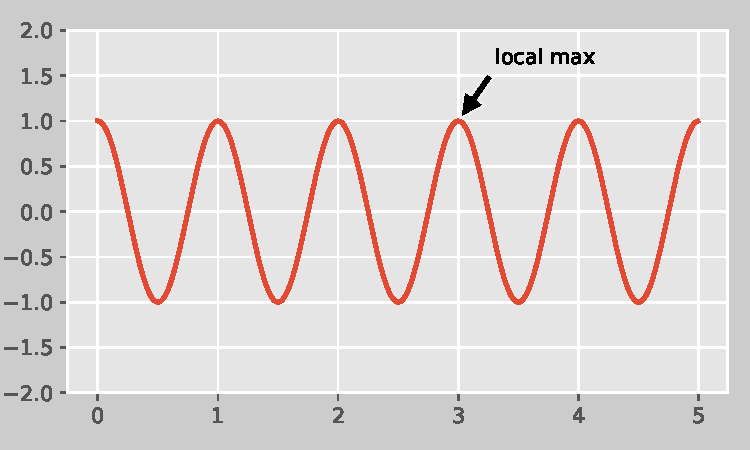
\includegraphics[width=0.9\linewidth]{python-visualization_files/figure-latex/unnamed-chunk-52-1} \end{center}

\hypertarget{argument-arrowprops}{%
\subsubsection{\texorpdfstring{argument \texttt{arrowprops}}{argument arrowprops}}\label{argument-arrowprops}}

\begin{enumerate}
\def\labelenumi{\arabic{enumi}.}
\tightlist
\item
  您可以通过在可选关键字参数\passthrough{\lstinline!arrowprops!}中提供箭头属性字典来启用箭头从文本到注释点的绘制.
\end{enumerate}

\begin{longtable}[]{@{}ll@{}}
\toprule
\endhead
arrowprops key & description\tabularnewline
width & 箭头的宽度\tabularnewline
frac & 箭头长度占头部的部分\tabularnewline
headwidth & 箭头头部的宽度,以点为单位\tabularnewline
shrink & move the tip and base some percent away from the annotated point and text\tabularnewline
**kwargs & any key for matplotlib.patches.Polygon, e.g., facecolor\tabularnewline
\bottomrule
\end{longtable}

\hypertarget{ux9ad8ux7ea7ux6807ux6ce8}{%
\subsection{高级标注}\label{ux9ad8ux7ea7ux6807ux6ce8}}

\hypertarget{annotating-with-text-with-box}{%
\subsubsection{Annotating with Text with Box}\label{annotating-with-text-with-box}}

\begin{enumerate}
\def\labelenumi{\arabic{enumi}.}
\tightlist
\item
  pyplot模块(或Axes类的text方法)中的text()函数,给定bbox关键字参数时在文本周围绘制一个框。
\item
  与文本关联的patch对象可以通过以下方式访问:
  \passthrough{\lstinline!bb = t.get\_bbox\_patch()!}
\item
  返回值是FancyBboxPatch的一个实例,可以像往常一样访问和修改patch属性,如facecolor、edgewidth等
\item
  要更改方框的形状,通过设置\textsubscript{boxstyle}方法。
\item
  \passthrough{\lstinline!pad!} :内边距
\end{enumerate}

\begin{lstlisting}[language=Python]
bbox_props = dict(boxstyle="rarrow,pad=0.3", fc="cyan", ec="b", lw=2)
t = ax.text(0.5, 0.5, "Direction", ha="center", va="center", rotation=45,
            size=15,
            bbox=bbox_props)
bb = t.get_bbox_patch()
bb.set_boxstyle("rarrow", pad=0.6)
\end{lstlisting}

\hypertarget{box-styles}{%
\subsubsection{box styles}\label{box-styles}}

\begin{longtable}[]{@{}lll@{}}
\toprule
Class & Name & Attrs\tabularnewline
\midrule
\endhead
Circle & circle & pad=0.3\tabularnewline
DArrow & darrow & pad=0.3\tabularnewline
LArrow & larrow & pad=0.3\tabularnewline
RArrow & rarrow & pad=0.3\tabularnewline
Round & round & pad=0.3,rounding\textsubscript{size}=None\tabularnewline
Round4 & round4 & pad=0.3,rounding\textsubscript{size}=None\tabularnewline
Roundtooth & roundtooth & pad=0.3,tooth\textsubscript{size}=None\tabularnewline
Sawtooth & sawtooth & pad=0.3,tooth\textsubscript{size}=None\tabularnewline
Square & square & pad=0.3\tabularnewline
\bottomrule
\end{longtable}

\hypertarget{fancybox-list}{%
\subsubsection{Fancybox list}\label{fancybox-list}}

\begin{lstlisting}[language=Python]
import matplotlib.pyplot as plt
import matplotlib.transforms as mtransforms
import matplotlib.patches as mpatch
from matplotlib.patches import FancyBboxPatch

styles = mpatch.BoxStyle.get_styles()
spacing = 1.2
figheight = (spacing * len(styles) + .5)
fig = plt.figure(figsize=(4 / 1.5, figheight / 1.5))
fontsize = 0.3 * 72

for i, stylename in enumerate(sorted(styles)):
    fig.text(0.5, (spacing * (len(styles) - i) - 0.5) / figheight, stylename,
              ha="center",
              size=fontsize,
              transform=fig.transFigure,
              bbox=dict(boxstyle=stylename, fc="w", ec="k"))

plt.show()
\end{lstlisting}

\begin{center}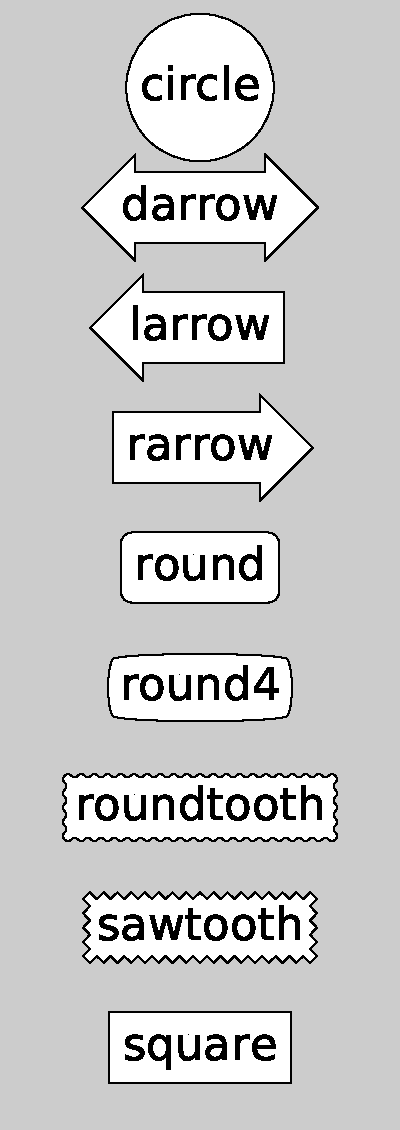
\includegraphics[width=0.9\linewidth]{python-visualization_files/figure-latex/unnamed-chunk-54-1} \end{center}

\hypertarget{annotating-with-arrow}{%
\subsubsection{Annotating with Arrow}\label{annotating-with-arrow}}

\begin{enumerate}
\def\labelenumi{\arabic{enumi}.}
\tightlist
\item
  绘制箭头需要几个步骤。

  \begin{itemize}
  \tightlist
  \item
    创建两点之间的连接路径。这是由connectionstyle键值控制的。
  \item
    如果patch对象是给定的(patchA \& patchB),路径会被裁剪以避免patch。
  \item
    路径可以进一步缩小到给定的像素量 (shrinkA \&
    shrinkB)
  \item
    路径转换为箭头patch对象,由箭头样式键值控制。
  \end{itemize}
\end{enumerate}

\hypertarget{ux793aux610fux56fe}{%
\subsubsection{示意图}\label{ux793aux610fux56fe}}

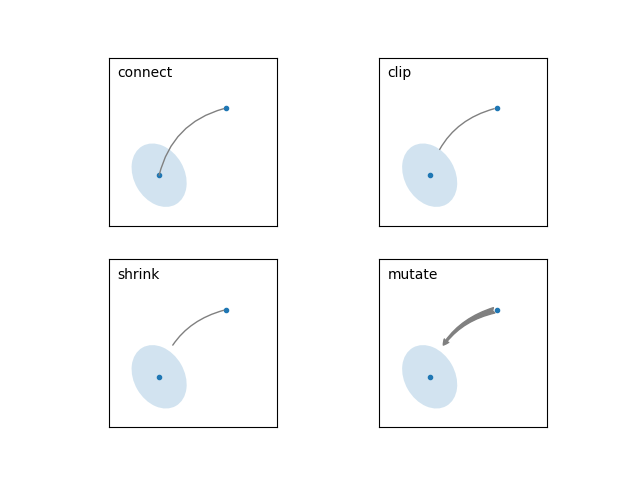
\includegraphics{images/annotate_explain.png}

\hypertarget{connectionstyle-key}{%
\subsubsection{\texorpdfstring{\texttt{connectionstyle} key}{connectionstyle key}}\label{connectionstyle-key}}

\begin{enumerate}
\def\labelenumi{\arabic{enumi}.}
\tightlist
\item
  两点之间连接路径的创建由connectionstyle键控制。下面的示例(有限地)演示了每种连接样式的行为。
\end{enumerate}

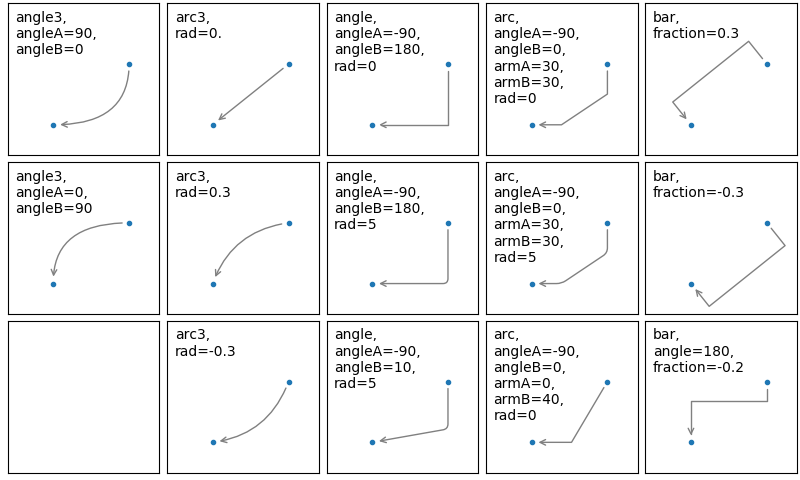
\includegraphics{images/connectionstyle_demo.png}

\hypertarget{arrowstyle}{%
\subsubsection{\texorpdfstring{\texttt{arrowstyle}}{arrowstyle}}\label{arrowstyle}}

\begin{enumerate}
\def\labelenumi{\arabic{enumi}.}
\tightlist
\item
  根据给定的\passthrough{\lstinline!arrowstyle!},连接路径(经过剪切和收缩)转变为一个箭头
\end{enumerate}

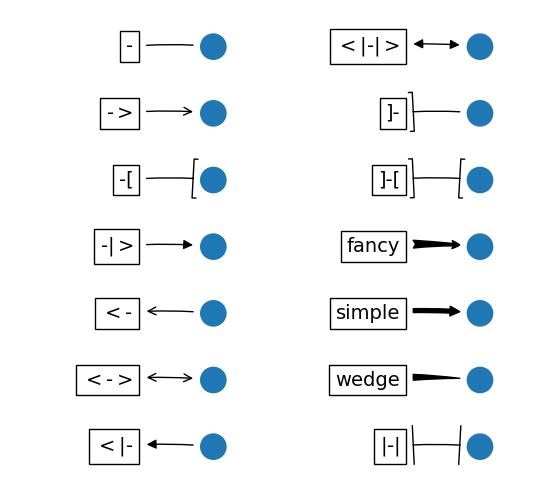
\includegraphics{images/fancyarrow_demo.png}

\hypertarget{using-connectionpatch}{%
\subsubsection{Using ConnectionPatch}\label{using-connectionpatch}}

\begin{enumerate}
\def\labelenumi{\arabic{enumi}.}
\item
  ConnectionPatch就像一个没有文本的注释。虽然在大多数情况下建议使用注释函数,但当您希望连接不同轴上的点时,\passthrough{\lstinline!ConnectionPatch!}非常有用。
\item
  \url{https://matplotlib.org/gallery/userdemo/connect_simple01.html}
\end{enumerate}

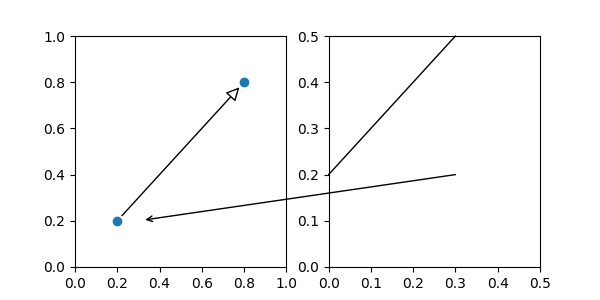
\includegraphics{images/connect_simple.png}

\hypertarget{zoom-effect-between-axes}{%
\subsubsection{Zoom effect between Axes}\label{zoom-effect-between-axes}}

\begin{enumerate}
\def\labelenumi{\arabic{enumi}.}
\item
  \passthrough{\lstinline!mpl\_toolkits.axes\_grid1.inset\_locator!} 定义了一些有效链接两个轴的patch对象
\item
  理解这些代码需要了解 mpl's transform 是如何工作的。
\item
  \url{https://matplotlib.org/gallery/subplots_axes_and_figures/axes_zoom_effect.html}
\end{enumerate}

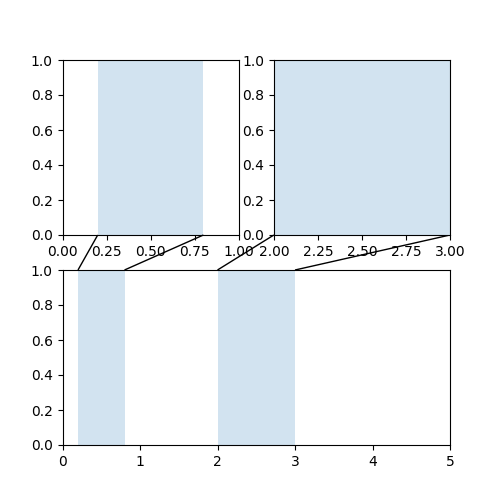
\includegraphics{images/axes_zoom_effect.png}

\hypertarget{mplot3dux5de5ux5177ux7bb1}{%
\section{mplot3d工具箱}\label{mplot3dux5de5ux5177ux7bb1}}

\hypertarget{how-is-mplot3d-different-from-mayavi}{%
\subsubsection{How is mplot3d different from MayaVi?}\label{how-is-mplot3d-different-from-mayavi}}

\begin{enumerate}
\def\labelenumi{\arabic{enumi}.}
\tightlist
\item
  MayaVi2 is a very powerful and featureful 3D graphing library. For
  advanced 3D scenes and excellent rendering capabilities, it is
  highly recommended to use MayaVi2.
\item
  mplot3d was intended to allow users to create simple 3D graphs with
  the same "look-and-feel" as matplotlib's 2D plots. Furthermore,
  users can use the same toolkit that they are already familiar with
  to generate both their 2D and 3D plots.
\end{enumerate}

\hypertarget{axes3d-object}{%
\subsubsection{\texorpdfstring{\texttt{Axes3D} object}{Axes3D object}}\label{axes3d-object}}

\begin{enumerate}
\def\labelenumi{\arabic{enumi}.}
\tightlist
\item
  An Axes3D object is created just like any other axes using the
  \passthrough{\lstinline!projection='3d'!} keyword.
\item
  Create a new matplotlib.figure.Figure and add a new axes to it of
  type Axes3D:
\end{enumerate}

\begin{lstlisting}[language=Python]
import matplotlib.pyplot as plt
from mpl_toolkits.mplot3d import Axes3D
fig = plt.figure()
ax = fig.add_subplot(111, projection='3d')
\end{lstlisting}

\hypertarget{ux4e00ux4e2aux4f8bux5b50}{%
\subsubsection{一个例子}\label{ux4e00ux4e2aux4f8bux5b50}}

\begin{lstlisting}[language=Python]
from mpl_toolkits.mplot3d import Axes3D
import numpy as np
import matplotlib.pyplot as plt

plt.rcParams['legend.fontsize'] = 10
fig = plt.figure()
ax = fig.gca(projection='3d')

# Prepare arrays x, y, z
theta = np.linspace(-4 * np.pi, 4 * np.pi, 100)
z = np.linspace(-2, 2, 100)
r = z**2 + 1
x = r * np.sin(theta)
y = r * np.cos(theta)

ax.plot(x, y, z, label='parametric curve')
ax.legend()

plt.show()
\end{lstlisting}

\begin{center}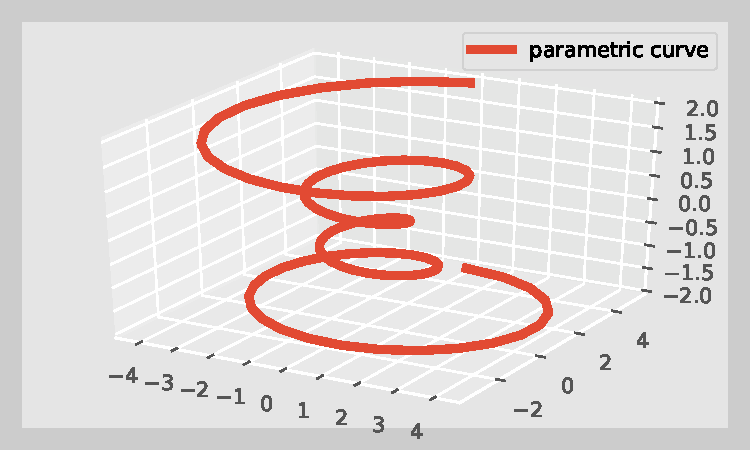
\includegraphics[width=0.9\linewidth]{python-visualization_files/figure-latex/unnamed-chunk-56-1} \end{center}

\hypertarget{ux652fux6301ux7684-3d-ux56feux5f62ux7c7bux578b}{%
\subsubsection{支持的 3D 图形类型}\label{ux652fux6301ux7684-3d-ux56feux5f62ux7c7bux578b}}

\begin{enumerate}
\def\labelenumi{\arabic{enumi}.}
\tightlist
\item
  \url{https://matplotlib.org/tutorials/toolkits/mplot3d.html\#sphx-glr-tutorials-toolkits-mplot3d-py}
\item
  Line plots: \passthrough{\lstinline!Axes3D.plot(self, xs, ys, *args, zdir='z', **kwargs)!}
\item
  Scatter plots:
  \passthrough{\lstinline!Axes3D.scatter(self, xs, ys, zs=0, zdir='z', s=20, c=None, depthshade=True, *args, **kwargs)!}
\item
  Wireframe plots:
  \passthrough{\lstinline!Axes3D.plot\_wireframe(self, X, Y, Z, *args, **kwargs)!}
\item
  Surface plots:
  \passthrough{\lstinline!Axes3D.plot\_surface(self, X, Y, Z, *args, norm=None, vmin=None, vmax=None, lightsource=None, **kwargs)!}
\item
  Tri-Surface plots:
  \passthrough{\lstinline!Axes3D.plot\_trisurf(self, *args, color=None, norm=None, vmin=None, vmax=None, lightsource=None, **kwargs)!}
\item
  Contour plots:
  \passthrough{\lstinline!Axes3D.contour(self, X, Y, Z, *args, extend3d=False, stride=5, zdir='z', offset=None, **kwargs)!}
\end{enumerate}

\hypertarget{ux652fux6301ux7684-3d-ux56feux5f62ux7c7bux578b-1}{%
\subsubsection{支持的 3D 图形类型}\label{ux652fux6301ux7684-3d-ux56feux5f62ux7c7bux578b-1}}

\begin{enumerate}
\def\labelenumi{\arabic{enumi}.}
\tightlist
\item
  Filled contour plots:
  \passthrough{\lstinline!Axes3D.contourf(self, X, Y, Z, *args, zdir='z', offset=None, **kwargs)!}
\item
  Polygon plots: \passthrough{\lstinline!Axes3D.add\_collection3d(self, col, zs=0, zdir='z')!}
\item
  Bar plots:
  \passthrough{\lstinline!Axes3D.bar(self, left, height, zs=0, zdir='z', *args, **kwargs)!}
\item
  Quiver:
  \passthrough{\lstinline!Axes3D.quiver(X, Y, Z, U, V, W, /, length=1, arrow\_length\_ratio=.3, pivot='tail', normalize=False, **kwargs)!}
\item
  2D plots in 3D
\item
  Text: \passthrough{\lstinline!Axes3D.text(self, x, y, z, s, zdir=None, **kwargs)!}
\item
  Subplotting:Having multiple 3D plots in a single figure is the same
  as it is for 2D plots. Also, you can have both 2D and 3D plots in
  the same figure.
\end{enumerate}

\hypertarget{ux5176ux4ed6ux5e38ux89c1ux4f5cux56feux5305}{%
\subsubsection{其他常见作图包}\label{ux5176ux4ed6ux5e38ux89c1ux4f5cux56feux5305}}

\begin{enumerate}
\def\labelenumi{\arabic{enumi}.}
\tightlist
\item
  Pandas is handy for simple plots but you need to be willing to learn
  matplotlib to customize.
\item
  Seaborn can support some more complex visualization approaches but
  still requires matplotlib knowledge to tweak. The color schemes are
  a nice bonus.
\item
  ggplot ggplot is a plotting system for Python based on R's ggplot2
  and the Grammar of Graphics. It is built for making profressional
  looking, plots quickly with minimal code.
\item
  Bokeh is an interactive visualization library for modern web
  browsers. It provides elegant, concise construction of versatile
  graphics, and affords high-performance interactivity over large or
  streaming datasets.
\item
  Mayavi: 3D scientific data visualization and plotting in Python.
\item
  Turtle graphics is a popular way for introducing programming to
  kids.
\end{enumerate}



\renewcommand\refname{参考文献}
\phantomsection %
\pdfbookmark{\refname}{reference}

\bibliography{./Bibfile.bib}




\end{document}
